\documentclass[handout,%
hyperref={unicode,colorlinks=true}]{beamer}
\usecolortheme{seahorse}
\usepackage{etex}   % lisää rekistereitä
%\usefonttheme{serif}
\usefonttheme[onlymath]{serif}     % serif vain matikkamoodiin
\usepackage[utf8]{inputenc}
\usepackage[T1]{fontenc}
\usepackage[finnish]{babel}
\usepackage{amsmath}
%\usepackage{amsfonts}
\usepackage{amssymb}
\usepackage{tikz}
\usepackage{framed}
\usepackage{alltt}
\usepackage{fancyvrb}
\usepackage{multirow}
\usepackage{mathtools}
\usepackage{multicol}
\usetikzlibrary{matrix,arrows,decorations.pathmorphing}
\usetikzlibrary{fadings,patterns,arrows}
\pgfmathsetmacro{\inf}{-2}
\pgfmathsetmacro{\sup}{2}
\tikzstyle{MyPlotStyle}=[domain=\inf:\sup,samples=100,smooth]
\usepgflibrary{arrows}

\usepackage{float}

\usepackage{lmodern}
\usepackage{microtype}
\usepackage{listings}
\lstset{
    language=[LaTeX]TeX,
    basicstyle=\ttfamily,%\footnotesize,
    commentstyle=\ttfamily,%\footnotesize,
    columns=fullflexible,
    keepspaces=true,
    backgroundcolor=\color{gray!20},
    escapechar=<>,
    morekeywords={\part,\chapter,\subsection,\subsubsection,\paragraph,\subparagraph,%
                  \middle,\theoremstyle,\eqref,\subsetneq},
    literate={ä}{{\"a}}1
             {Ä}{{\"A}}1
             {ö}{{\"o}}1
             {Ö}{{\"O}}1
}
\lstdefinelanguage{BibTeX}
    {keywords={%
        @article,@book,@collectedbook,@conference,@electronic,@ieeetranbstctl,%
        @inbook,@incollectedbook,@incollection,@injournal,@inproceedings,%
        @manual,@mastersthesis,@misc,@patent,@periodical,@phdthesis,@preamble,%
        @proceedings,@standard,@string,@techreport,@unpublished%
    },
    comment=[l][\itshape]{@comment},
    sensitive=false,
}

\newcommand{\cns}[1]{\texttt{#1}}   % vakioille yms.
\newcommand{\newterm}[1]{\textit{#1}}

\newcounter{harkka}
\newtheorem{lause}{Lause}
\newtheorem*{huom}{Huomautus}
\newcounter{laskuri}
\newtheorem{trma}{Teoreema}[laskuri]
\newtheorem{prop}[trma]{Propositio}
\theoremstyle{remark}
\newtheorem{harj}{Harjoitus}[section]

\newenvironment{fframe}
    {\begin{frame}[fragile,environment=fframe]}
    {\end{frame}}

\newtheorem*{esim}{Esimerkki}
\newtheorem*{ratk}{Ratkaisuehdotus}
\newtheorem*{thmextra}{Lisätieto}
\newenvironment{extra}{\begin{thmextra}\footnotesize}{\end{thmextra}}
\newenvironment{serif}{\fontfamily{lmr}\selectfont}{}
\usepackage{ragged2e}   % \justifying
\newenvironment{sample}{\begin{framed}\justifying\begin{serif}}{\end{serif}\end{framed}}



%Matriisien säätö:
\makeatletter
\renewcommand*\env@matrix[1][*\c@MaxMatrixCols c]{%
    \hskip -\arraycolsep
    \let\@ifnextchar\new@ifnextchar
\array{#1}}
\makeatother

\newcommand{\numeroi}{\stepcounter{harkka}\arabic{harkka}}
\newcommand{\vaihto}{\\[1em]}
\newcommand{\R}{\mathbb{R}\,}
\newcommand{\N}{\mathbb{N}\,}
\newcommand{\Z}{\mathbb{Z}\,}
\newcommand{\Q}{\mathbb{Q}\,}
\providecommand{\C}{}               % XeTeX:illä tämä on jokin aksenttikomento
\renewcommand{\C}{\mathbb{C}\,}
\newcommand{\abs}[1]{\left|#1\right|}
\newcommand{\va}{\bar{a}}
\newcommand{\vb}{\bar{b}}
\newcommand{\vw}{\bar{w}}
\newcommand{\vv}{\bar{v}}
%\newcommand{\abs}[1]{\left|#1\right|}
%\newcommand{\BibTeX}{\textsc{Bib}\negthinspace\TeX}
\newcommand{\BibTeX}{Bib\negthinspace\TeX}  % textsc toimii lmodernilla, mutta näyttää pahalta...
\newcommand{\TikZ}{Ti\textit{k}Z}
%\newcommand{\bino}[2]{(x-#1)^{#2}}
\newcommand{\bino}[3]{\binom{#1}{#3}{#2}^{#3}\left(1-#2\right)^{#1-#3}}
\setbeamertemplate{theorems}[numbered]
\newcommand{\set}[1]{ \{ #1 \} }

\title{\LaTeX}



\AtBeginSection{
    \begin{frame}
        \frametitle{Suunnitelma}
        \begin{columns}[t]
            \column{5cm}
            \tableofcontents[sections={1-2},sectionstyle=show/shaded,subsectionstyle=show/show/shaded,subsubsectionstyle=show/show/hide]
            \column{5cm}
            \tableofcontents[sections={3-4},sectionstyle=show/shaded,subsectionstyle=show/show/shaded,subsubsectionstyle=show/show/hide]
        \end{columns}
    \end{frame}
}
\AtBeginSubsection{
    \begin{frame}
        \frametitle{Suunnitelma}
        \tableofcontents[sectionstyle=show/hide,subsectionstyle=show/shaded/hide,subsubsectionstyle=show/show/shaded]
    \end{frame}
}

\begin{document}
\begin{frame}
    \titlepage
\end{frame}
%\begin{frame}
%    \frametitle{Kurssisuunnitelma}
%    \tableofcontents
%\end{frame}

\section{1. kerta}



%\begin{itemize}
%\item 1. kerta
%\begin{itemize}
%\item Mikä \LaTeX\ on?
%\item Dokumentin rakenne ja luominen
%\item Syntaksi eli ''kielioppi''
%\item Virheilmoitukset
%\item Tekstin muokkaaminen
%\item Matematiikkatila
%\item Numeroidut kaavat
%\end{itemize}
%\item 2. kerta
%\begin{itemize}
%\item Lauseympäristöt
%\item Otsikot
%\item Lauseympäristöjen numerointi
%\item Listat
%\item Omat komennot
%\end{itemize}
%\item 3. kerta
%\begin{itemize}
%\item Taulukot
%\item Kuvien liittäminen
%\item Kuvien piirtäminen
%\item Pakettien hakeminen
%\end{itemize}
%\item 4. kerta
%\begin{itemize}
%\item Sisäiset viittaukset
%\item Lähdeluettelo
%\item Sisällysluettelo ja hakemisto
%\item Kansilehti
%\item Tyylittely
%\end{itemize}
%\end{itemize}

\subsection{Intro}
\begin{frame}
    \frametitle{Mikä \LaTeX\  on?}
    \begin{itemize}[<+->]
        \item Tekstin ladontajärjestelmä
        \item Matemaattisen tekstin tuottamista varten
        \item Kehitetty \TeX -kielen päälle (Leslie Lamport)
        \item Laajalti käytössä ympäri maailman
        \item Merkittävästi erilainen kuin WYSIWYG-järjestelmät
            %ESIMERKKINÄ LAITOKSEN TUTKIELMAPOHJA
    \end{itemize}
\end{frame}


\subsection{Dokumentin rakenne}
\begin{frame}[fragile]
    \frametitle{Dokumentin rakenne ja luominen}
    \LaTeX-dokumentit tuotetaan tällä kurssilla helppokäyttöisellä Texmaker-ohjelmalla.
    \pause
    \vaihto
    Texmakeriin kirjoitetaan dokumentin koodi ja lopuksi tiedosto \newterm{käännetään} eli \newterm{ajetaan} varsinaiseksi (PDF- tai DVI-) tiedostoksi. Kääntämisen hoitaa \LaTeX\ käyttäjältä piilossa.
    \pause
    \vaihto
    Tarvittavat ohjelmat omalle koneelleen löytää esimerkiksi Matematiikan laitoksen sivujen kautta osoitteesta
    \url{http://wiki.helsinki.fi/pages/viewpage.action?pageId=62428926}
    \pause
    \vaihto
    Kaikkein helpoimmin kuitenkin pääsee alkuun käyttämällä jotain online-ympäristöä kuten esimerkiksi Overleaf (\url{https://www.overleaf.com/}). Tällöin mitään ohjelmia ei tarvitse asentaa eikä tiedostoja siirrellä koneiden välillä.
\end{frame}

\begin{frame}[fragile]
        \begin{harj}
        \begin{itemize}
            \item Avaa Texmaker ja luo uusi tiedosto
            \item Tallenna se muodossa \verb-nimi.tex- johonkin tätä kurssia varten luomaasi kansioon
            \item Kirjoita tiedostoon seuraavat rivit:
                \begin{verbatim}
\documentclass{article}
\begin{document}
Huhuu!
\end{document}
                \end{verbatim}
            \item Aja tiedosto PDFLaTeX:illa
            \item Valitse View PDF
        \end{itemize}
    \end{harj}

\end{frame}

\begin{frame}[fragile]
    \frametitle{Dokumentin rakenne ja luominen}
    \LaTeX-dokumentti koostuu kahdesta osasta: \newterm{esittelyosasta}, joka sisältää tarpeellisia asetuksia ja \newterm{sisällöstä} eli varsinaisesta dokumentista.
    \pause
    \begin{itemize}[<+->]
        \item Tiedosto ja samalla esittelyosa aloitetaan komennolla \lstinline+\documentclass{...}+, jolla valitaan dokumenttiluokka (\cns{article})
        \item Esittelyosaan lisätään komentoja tarpeen mukaan
        \item Komento \lstinline+\begin{document}+ aloittaa itse dokumentin ja lopettaa esittelyosan
        \item Komento \lstinline+\end{document}+  lopettaa dokumentin eikä sen perään kirjoitettuja rivejä käännetä.
        \item Varsinainen työn sisältö kirjoitetaan siis komentojen \lstinline+\begin{document}+  ja  \lstinline+\end{document}+  väliin.
    \end{itemize}
    (Vrt. edellinen harjoitus!)
\end{frame}

\begin{frame}[fragile]
    \frametitle{Dokumentin rakenne ja luominen}
    Esittelyosassa eli heti komennon \lstinline+\documentclass{}+  jälkeen valitaan käytettävät paketit ja asetukset. \pause Ääkkösiä ja suomalaista tavutusta varten otetaan käyttöön tietyt \cns{inputenc}-, \cns{fontenc}- ja \cns{babel}-paketit:\pause
        \begin{harj}
        Tee dokumenttiisi seuraavat muutokset (älä siis luo uutta tiedostoa):
        %\usepackage[ansinew]{inputenc}
        \begin{Verbatim}[frame=single]
\documentclass[a4paper]{article}
\usepackage[utf8]{inputenc}
\usepackage[T1]{fontenc}
\usepackage[finnish]{babel}
\usepackage{geometry}
\begin{document}
Öö häh? Herätys!
\end{document}
        \end{Verbatim}
    \end{harj}

\end{frame}

\begin{frame}[fragile]
    \begin{extra}
        \begin{itemize}
            \item Käyttämällä \cns{inputenc}-pakettia \LaTeX{} lukee \cns{.tex}-tiedoston \cns{utf8}-koodattuna, jolloin esim. ä voidaan kirjoittaa tiedostoon sellaisenaan eikä muodossa \lstinline-\"a-. Tämä vaatii, että käyttämäsi editori tallentaa tiedoston \cns{utf8}-koodattuna. Esim. Texmaker ja Overleaf tekevät niin oletuksena. Jos ääkköset eivät toimi oikein, niin ongelma on todennäköisesti siinä, että tiedosto on koodattu eri tavalla kuin sitä yritetään lukea. Jos ääkköset eivät toimi, voit yrittää kirjoittaa \cns{[utf8]} sijaan esim. \cns{[latin1]}, \cns{[ansinew]} tai \cns{[applemac]}. Paras olisi kuitenkin käyttää \cns{[utf8]}:aa ja yrittää saada editori tallentamaan tässä muodossa.
            \item Paketti \cns{fontenc} ottaa käyttöön laajemmat fontit, jolloin esim. ä tulostetaan yhtenä merkkinä eikä niin, että merkit a ja \"{} kirjoitetaan päällekkäin. Tällöin vaikkapa tavutus ja pdf-haku saadaan toimimaan oikein.
            \item Lopuksi \cns{babel} asettaa dokumentin kielen suomeksi ottamalla käyttöön suomalaiset tavutussäännöt ym.
        \end{itemize}
    \end{extra}
\end{frame}

\begin{frame}[fragile]
        \begin{harj}
        Kopioi työhösi pari sivullista suomenkielistä tekstiä esimerkiksi Wikipediasta (vältä erikoismerkkejä). Aja tiedosto. Varmista vielä ääkkösten ja tavutuksen toimiminen. Miten kappalejaon kanssa käy?
    \end{harj}

\end{frame}

\begin{frame}[fragile]
    Edellä mainitut paketit ovat esimerkkejä \newterm{makropaketeista}, joilla \LaTeX in eli latojan toimintaan voi vaikuttaa. 
    \pause
    Matemaattista tekstiä varten on vielä syytä ottaa käyttöön muutama lisäpaketti. 
        \begin{harj}
        Ota käyttöön paketit\footnote{ams tulee sanoista American Mathematical Society}
        \begin{center}
            \cns{amsmath},\quad \cns{amsthm}\quad ja\quad \cns{amssymb}
        \end{center}
        lisäämällä dokumenttisi esittelyosaan seuraavat komennot:
        \begin{lstlisting}
\usepackage{amsmath}
\usepackage{amsthm}
\usepackage{amssymb}<>
        \end{lstlisting}
        \pause
        Nämä sisältävät fontteja, symboleita ja muuta matemaattisen tekstin kirjoittamiselle tarpeellista. Paketti \cns{amsmath} on ladattava ennen \cns{amsthm}-pakettia.
    \end{harj}

\end{frame}

\begin{frame}[fragile]
    \frametitle{Syntaksi eli ''kielioppi''}
    \LaTeX in toimintaa ohjataan komennoilla. \pause Niillä tuotetaan esimerkiksi matemaattisia symboleita, korostetaan tekstin osia, luodaan otsikoita, piirretään kuvia, määritellään asetuksia jne.  \pause
    \begin{framed}
        Komennot alkavat aina kenoviivalla \lstinline-\-
    \end{framed}
    \pause
    Komentoja voi tarvittaessa etsiä esimerkiksi oppaista \begin{scriptsize}
        \url{http://www.ntg.nl/doc/hellgren/lyhyt2e.pdf}
    \end{scriptsize},
    \begin{scriptsize}
        \url{http://en.wikibooks.org/wiki/LaTeX}
    \end{scriptsize} ja
    \begin{scriptsize}
        \url{http://www.rri.res.in/~sanjib/latex/ltx-2.html}
    \end{scriptsize}
\end{frame}


\subsection{Syntaksi}
\begin{frame}[fragile]
    \frametitle{Syntaksi}
    %Edellä on jo tutustuttu komentoihin \verb-\documentclass{}-, \verb-\begin{}...\end{}-, \verb-\usepackage[]{}- jne. Ne ovat esimerkkejä komennoista, jotka
    Komennot tarvitsevat usein \newterm{argumentin} (lisämääreen). \pause Se kirjoitetaan komennon perään
    \begin{itemize}[<+->]
        \item aaltosulkuihin \lstinline-{}-, kun argumentti on pakollinen
        \item hakasulkuihin \lstinline-[]-, kun argumentti on valinnainen
            %\item Pakollinen argumentti on komennon perässä aaltosuluissa \verb-{}-
            %\item Valinnainen argumentti on komennon perässä hakasuluissa \verb-[]-
    \end{itemize}
    \pause
    Komennolla voi olla yksi tai useampi pakollinen argumentti ja lisäksi yksi tai useampi valinnainen argumentti. \pause Toisilla komennoilla ei ole ainuttakaan argumenttia.
\end{frame}

\begin{frame}[fragile]
    \frametitle{Syntaksi}
    Esimerkiksi 
    \begin{itemize}[<+->]
        \item Komennoilla \lstinline-\cup- ja \lstinline-\cap- ei ole yhtään argumenttia (joukkojen yhdiste ja leikkaus)
        \item Komennolla \lstinline-\sqrt[]{}- on yksi valinnainen ja yksi pakollinen argumentti (valinnainen on juuren kertaluku, pakollinen juurrettava luku. Jos valinnainen argumentti puuttuu, \LaTeX\ tulkitsee neliöjuureksi)
        \item Komennolla \lstinline-\documentclass[]{}- on myös valinnainen argumentti, jolla voi valita mm. kirjain- ja paperikoon
        \item Komennolla \lstinline-\frac{}{}- on kaksi pakollista argumenttia (murtoluvun osoittaja ja nimittäjä)
    \end{itemize}
    %Komentoja ja niiden selityksiä voi etsiä esimerkiksi osoitteista
    %\begin{itemize}
    %\item \url{http://www.rri.res.in/~sanjib/latex/ltx-2.html}
    %\end{itemize}
    %PAREMPI LINKKI
    \pause
    Argumenttien järjestyksen ja määrän kanssa on oltava tarkka!
\end{frame}

\begin{frame}[fragile]
    \frametitle{Syntaksi}
    Muotoa 
    \begin{lstlisting}
\begin{ympäristön nimi}
    ...
\end{ympäristön nimi}<>
    \end{lstlisting}
    olevilla komentopareilla käytetään ns. \newterm{ympäristöjä}. \pause Näitä voivat olla esimerkiksi lauseet, määritelmät, listat ja taulukot. \pause
    \vaihto Ympäristölläkin voi olla nimen lisäksi muita pakollisia tai valinnaisia argumentteja, kuten tieto taulukon sarakkeiden lukumäärästä tai kuvan toivotusta sijainnista. \pause
    \vaihto
    Kurssin aikana opetellaan käyttämään muutamia tarpeellisia ympäristöjä ja luomaan omia komentoja.
\end{frame}

\begin{frame}[fragile]
    \frametitle{Erikoismerkeistä}
    Jotkin erikoismerkit on varattu \LaTeX in käyttöön:
    \begin{itemize}[<+->]
        \item \lstinline-%- aloittaa kommenttirivin
        \item \lstinline-$- aloittaa ja lopettaa tavallisen matematiikkatilan
        \item \lstinline-\- aloittaa komennon (komento \lstinline-\\- katkaisee rivin)
        \item \lstinline-&- on käytössä kun rivejä järjestetään kohdakkain
        \item \lstinline-{- ja \lstinline-}- ovat komennon argumentin ympärille tulevat merkit
    \end{itemize}\pause
    Jotta erikoismerkin saisi näkyviin lopullisessa työssä, on käytettävä komentoa:
    \begin{table}[H]
        \begin{tabular}{ccc}
            Komento & & Tulostus\\
            \hline
            \verb-\%- & & \%\\
            \verb-\$- & & \$\\
%            \verb-\backslash- & & \(\backslash\)\\
            \verb-\textbackslash- & & \textbackslash\\
            \verb-\&- & & \&\\
            \verb-\{\}- & & \{\}
        \end{tabular}
    \end{table}
\end{frame}

\begin{frame}[fragile]
        \begin{harj}
        Kolme peräkkäistä pistettä saa komennolla \lstinline-\dots-. Kokeile, miten lopputulokset eroavat, jos kirjoitat pisteet itse.  Kirjoita sitten seuraava:
        \begin{sample}
            Erikoismerkkejä ovat mm. \%, \$ ja \&. Merkkijonon \textbackslash textbackslash tuottaminen onnistuu näin\dots
        \end{sample}
    \end{harj}

        \begin{harj}
        Kommenttirivin avulla koodin sekaan voi kirjoittaa selkeyttäviä huomautuksia, jotka eivät tule näkyviin lopulliseen työhön. Kommenttirivi aloitetaan merkillä \verb-%- ja päätetään rivinvaihtoon. 
        \vaihto
        Kirjoita koodin sekaan esimerkiksi rivi
        \begin{Verbatim}[frame=single]
%Tämä rivi ei tule näkyviin lopullisessa työssä.
        \end{Verbatim}
        ja testaa, pitääkö väite paikkansa.
    \end{harj}

\end{frame}

\begin{frame}
    \frametitle{Virheilmoitukset}
    Tiedoston ajamisen jälkeen Texmakerin alareunaan saattaa ilmestyä sinisiä ja punaisia viestejä.\pause
    \begin{itemize}[<+->]
        \item \textcolor{blue}{Siniset} viestit ovat varoituksia ulkonäöllisista seikoista
        \item \textcolor{red}{Punaiset} viestit ovat kääntämisen estäviä virheitä
    \end{itemize}\pause
    Punaisten virheilmoitusten kanssa on pakko olla tarkka -- virheet tulee korjata heti!
    \vaihto
    \pause
    Virheilmoituksesta on pääteltävissä jotain sattuneesta virheestä, mutta tämä vaatii totuttelua. 
    \pause Yleensä kyseessä on jonkin komennon väärinkirjoitus, puuttuva aaltosulku tai muu pieni yksityiskohta.
    \vaihto
    \pause Virheilmoituksia saattaa tulla valtavasti vaikka kyse olisi yksittäisestä ongelmasta!
\end{frame}


\subsection{Otsikot ja korostukset}
\begin{frame}[fragile]
    \frametitle{Otsikot}
    Teksti jäsennetään ja otsikoidaan komennoilla 
    \begin{itemize}[<+->]
        \item \lstinline-\part{Osan otsikko}-
        \item \lstinline-\chapter{Luvun otsikko}- (vain luokissa \cns{book} ja \cns{report})
        \item \lstinline-\section{Osion otsikko}-
        \item \lstinline-\subsection{Aliosion otsikko}-
        \item \lstinline-\subsubsection{Alialiosion otsikko}-
        \item \lstinline-\paragraph{Kappaleen otsikko}-
        \item \lstinline-\subparagraph{Alikappaleen otsikko}-
    \end{itemize} \pause
    %Dokumenttiluokissa \verb-report- ja \verb-book- on käytössä myös \verb-\chapter-, alilukunaan \verb-\section- jne.
    Neljän karkeimman tason otsikot numeroidaan automaattisesti. \pause Numeroinnin saa pois lisäämällä merkin \lstinline-*- komennon perään, siis esimerkiksi 
    \begin{lstlisting}
\section*{numeroimaton otsikko}<>
    \end{lstlisting}
\end{frame}

\begin{frame}
        \begin{harj}
        \begin{itemize}
            \item Jaa tekstisi neljään numeroituun osioon
            \item Jaa ensimmäinen osio lisäksi muutamaksi ali- ja alialiosioksi
            \item Jätä ainakin yksi alialiosio numeroimatta
            \item Nimeä kaikki osiot
        \end{itemize}
        Tee ensimmäisen kerran harjoitukset ensimmäiseen osioon, toisen kerran harjoitukset toiseen osioon jne. 
    \end{harj}

\end{frame}

\begin{frame}[fragile]
    \frametitle{Tekstin muokkaaminen}
    Tekstieditorissa eli Texmaker-ohjelmassa käytetty fontti tai tekstin suuruus eivät vaikuta lopulliseen työhön, vaan kaikki ulkoasulliset muutokset on tehtävä komennoilla.% (Isot/pienet kirjaimet toimivat kuitenkin sellaisenaan.)
    \vaihto\pause
    Erityisesti kannattaa huomata, että tekstiä kirjoittaessa
    \begin{itemize}[<+->]
        \item peräkkäiset välilyönnit tulostuvat yhdeksi välilyönniksi
        \item myös yksittäinen rivinvaihto tulkitaan välilyönniksi
        \item tyhjä rivi (yksi tai useampi) aloittaa uuden kappaleen
    \end{itemize}
    \pause
    Erikokoisia välilyöntejä varten on omia komentojaan, kuten esimerkiksi \lstinline-\,- , \lstinline-\quad- ja \lstinline-\qquad-.
    \vaihto\pause Pystysuunnassa tyhjää tilaa saa sanomalla esim. \lstinline-\vspace{2.5cm}-. Yhden tyhjän rivin saa komennolla \lstinline-\vspace{\baselineskip}-.
\end{frame}

%\begin{frame}[fragile]
%\frametitle{Tekstin muokkaaminen}
%Koodin sekaan voi kirjoittaa ns. kommenttirivejä, joita ei huomioida käännettäessä eikä siis näytetä lopullisessa työssä. Kommentti alkaa merkillä \verb-%- ja päättyy rivinvaihtoon. Kommentointi kannattaa!
%\vaihto
%Tekstin tasauksen voi valita komennoilla \verb-\centering-, \verb-\flushleft-, \verb-\flushright-. 
%\vaihto
%
%\end{frame}

\begin{frame}[fragile]
    \frametitle{Tekstin muokkaaminen}
    Kirjainkokoa voi kesken tekstin muuttaa lukuisilla komennoilla kuten \lstinline-\huge-, \lstinline-\tiny-, ja \lstinline-\normalsize-, jotka vaikuttavat kunnes kokoa taas muutetaan. 
    \vaihto\pause
    Tekstin \textbf{lihavointi} onnistuu manuaalisesti komennolla \lstinline-\textbf{lihavoitava teksti}-, \textit{kursivointi} komennolla \lstinline-\textit{kursivoitava teksti}- ja \underline{alleviivaus} komennolla \lstinline-\underline{alleviivattava teksti}-. Alleviivaus rikkoo tavutuksen ym., joten ahkeran alleviivaajan kannattaa tutustua esim. \cns{ulem}-pakettiin.
    \vaihto\pause
    Sanojen korostamiseen kannattaa kuitenkin käyttää komentoa \verb-\emph{korostettava teksti}-, joka muuttaa fontin sopivaksi kontekstin perusteella!
\end{frame}

\begin{frame}[fragile]
    \frametitle{Tekstin muokkaaminen}
    Tekstin keskittäminen onnistuu ympäristön \verb-center- avulla:
    \begin{lstlisting}
\begin{center}
    ...keskitetty teksti...
\end{center}<>
    \end{lstlisting}
    Tällä tavoin keskitetyn tekstin ylä- ja alapuolelle jää hieman tyhjää tilaa. \vaihto\pause
    Oikeaan tai vasempaan laitaan tasattua tekstiä saa halutessaan ympäristöillä \cns{flushright} ja \cns{flushleft}.

\end{frame}
\begin{frame}
        \begin{harj}
        Valitse dokumentistasi muutama rivi tekstiä ja keskitä se tai tasaa oikeaan laitaan. Muokkaa sitten tasattua tekstiä käyttämällä erilaisia kirjainkokoja ja korostuksia. Esimerkiksi siis jotain seuraavanlaista:
        \begin{sample}
            \begin{flushright}
                Tämä teksti on normaalikokoista, \tiny mutta tämä pientä ja \huge tämä suurta \normalsize. Tähän laitan suuren välin: \qquad, tähän vähän pienemmän: \quad ja \emph{tätä tekstiä taas haluan korostaa!}
            \end{flushright}
        \end{sample}
    \end{harj}

\end{frame}


\subsection{Matemaattinen teksti}
\begin{frame}[fragile]
    \frametitle{Matematiikkatila}
    Matemaattisia ilmaisuja saa tekstin sekaan käyttämällä komentoja \lstinline+\(+  
    ja \lstinline+\)+. \pause Esimerkiksi rivi
    \begin{lstlisting}
Yhtälöt \(x^2+y^2-2=0\) ja \(y=2x+1\) toteutuvat 
samanaikaisesti tasan kahdessa tason pisteessä.<>
    \end{lstlisting}
    \pause
    tulostuu riviksi 
    \begin{sample}
        Yhtälöt \(x^2+y^2-2=0\) ja \(y=2x+1\) toteutuvat samanaikaisesti tasan kahdessa tason pisteessä.
    \end{sample} 
    \pause
    Huomaa, että matematiikkatilassa kirjaimet tulostuvat erilailla, kuin muussa tekstissä. 
    %Huomaa myös, että 
    %\[
    %\verbö\(2x+3=4\)ö
    %\]
    %tuottaa yhtälön \(2x+3=4\) \pause ja komento 
    %\[
    %\verbö\(x^3+\sqrt{2}x^2+1=0\)ö
    %\]
    %yhtälön \(x^3+\sqrt{2}x^2+1=0\). \pause Tätä kutsutaan matematiikkatilaksi.
\end{frame}

\begin{frame}[fragile]
        \begin{harj}
        Tuota seuraava lause dokumenttiisi:
        \begin{sample}
            Vaihdannaisessa renkaassa pätee \((a+b)^2=a^2+2ab+b^2\). Jos siis \(2ab\neq0\), niin \((a+b)^2\neq a^2+b^2\). 
        \end{sample}
        Erisuuruuden saat komennolla \verb-\neq-.
    \end{harj}

\end{frame}

\begin{frame}[fragile]
    \frametitle{Kaavarivi}
    Kun matemaattinen ilmaisu halutaan yksinkertaisesti omalle kaavarivilleen, se kirjoitetaan komentojen \lstinline-\[- ja \lstinline-\]- väliin.
    \pause
    Esimerkiksi 
    \begin{lstlisting}
Toisen asteen yhtälön \(ax^2 + bx + c = 0\) ratkaisu
saadaan kaavasta
\[
    x = \frac{-b \pm \sqrt{b^2 - 4ac}}{2a}.
\]<>
    \end{lstlisting}
    tuottaa seuraavanlaisen esityksen:
    \pause
    \begin{sample}
        Toisen asteen yhtälön \(ax^2 + bx + c = 0\)
        ratkaisu saadaan kaavasta
        \[
            x = \frac{-b \pm \sqrt{b^2 - 4ac}}{2a}.
        \]
    \end{sample}
\end{frame}

\begin{frame}[fragile]
        \begin{harj}\label{rajaArvo}
        Tuota seuraava dokumenttiisi:
        \begin{sample}
            Funktion \(f\colon \R\to \R\) derivaatta pisteessä \(x_0\in\R\) on
            \[
                f'(x_0)=\lim_{x\to x_0}\frac{f(x)-f(x_0)}{x-x_0},
            \]
            mikäli raja-arvo on olemassa.
        \end{sample}
    \end{harj}

\end{frame}

\begin{frame}[fragile]
        \begin{harj}
        Tuota seuraava dokumenttiisi:
        \begin{sample}
            Jos \(F\) on \(\sigma\)-algebra ja \(A_i\in F\) kaikilla \(i= 1,2,\dots\), niin 
            \[
                \bigcup_{i=1}^{\infty} A_i\in F.
            \]
        \end{sample}
        Tarvitset mm. komentoja \lstinline-\sigma-, \lstinline-\in-, \lstinline-\bigcup- ja \lstinline-\infty-. Ala- ja yläindeksit kirjoitetaan merkkien \lstinline-_- ja \lstinline-^- avulla (jos indeksiin halutaan enemmän kuin yksi merkki, se täytyy laittaa aaltosulkeisiin kuten edellisessä tehtävässä). 
    \end{harj}

\end{frame}

\begin{frame}[fragile]
    Yleisimpiä matemaattisia symboleita löytää Texmakerin vasempaan laitaan avautuvista valikoista. Muuten niitä voi etsiä esim. seuraavista osoitteista:
    \begin{scriptsize}
        \begin{itemize}
            \item \url{http://www.tex.ac.uk/tex-archive/info/symbols/comprehensive/symbols-a4.pdf}
            \item \url{http://detexify.kirelabs.org/classify.html}
        \end{itemize}
    \end{scriptsize}
        \begin{harj}
        Selvitä, miten voit tuottaa vektorimerkinnät \(\bar{v}\), \(\bar{w}\) ja \(\overline{AB}\). Kirjoita seuraava:
        \begin{sample}
            Vektoreiden \(\bar{v}=\overline{AB}\) ja \(\bar{w}=\overline{CD}\) ristitulo \(\bar{v}\times\bar{w}\) on kohtisuorassa kumpaakin vektoria vastaan. Vektoreiden pistetulo \(\bar{v}\cdot\bar{w}\) on sen sijaan reaaliluku.
        \end{sample}
    \end{harj}


\end{frame}



\section{2. kerta}


\subsection{Matemaattinen teksti}
\begin{frame}[fragile]
    \frametitle{Sulut}
    Varsinkin kaavariville kirjoitettaessa monet symbolit ovat huomattavan kookkaita. Sulut tulostuvat automaattisesti oikean kokoisina kun niille käytetään komentoja pelkkien merkkien \lstinline-(- ja \lstinline-)- sijaan. \vaihto
    \begin{tabular}{cc|cc}
        %\multicolumn{2}{c}{Vasen}&\multicolumn{2}{c}{Oikea}\\
        Komento & Tulostus & Komento & Tulostus\\
        \hline
        \lstinline-\left(- & \(\left(\right.\) & \lstinline-\right)-& \(\left.\right)\)\\
        \lstinline-\left[- & \(\left[\right.\) & \lstinline-\right]-& \(\left.\right]\)\\
        \lstinline-\left\lbrace- & \(\left\lbrace\right.\) & \lstinline-\right\rbrace- & \(\left.\right\rbrace\)\\
        \lstinline-\left\langle- & \(\left\langle\right.\) & \lstinline-\right\rangle- & \(\left.\right\rangle\)\\
        \lstinline-\left|- & \(\left|\right.\) & \lstinline-\right|- & \(\left.\right|\)\\
    \end{tabular}
    \vaihto
    Jokaista \lstinline-\left--alkuista komentoa täytyy seurata \lstinline-\right--alkuinen komento, vähintään \lstinline-\right.- , joka ei tulosta mitään. Samoin \lstinline-\right--alkuista komentoa on edellettävä \lstinline-\left--alkuinen komento, vähintään \lstinline-\left.- . 
\end{frame}

\begin{frame}[fragile]
        \begin{harj}
        Tuota seuraava dokumenttiisi:
        \begin{sample}
            Todista seuraava yhtälö:
            \[
                \left\lbrace 2^n \,\middle|\, n\in\Z\right\rbrace=\left\lbrace \left(\frac{1}{2}\right)^{-n}\,\middle|\, n\in\Z\right\rbrace
            \]
        \end{sample}
        Komennolla \lstinline-\middle|- saat pystyviivan automaattisesti oikean kokoisena ja komennolla \lstinline-\,- hieman ylimääräistä väliä niiden ympärille. Tehtävästä \ref{rajaArvo} saat apua symboleiden \(\in\) ja \(\Z\) luomiseen.
    \end{harj}

\end{frame}
\begin{frame}[fragile]
        \begin{harj}
        Lisää dokumenttiisi jokin lainaus käyttäen \verb-quote--, \verb-\quotation-- tai \verb-verse--ympäristöä. 
    \end{harj}

\end{frame}

\begin{frame}[fragile]
    \frametitle{Vanhoja tapoja}

    \begin{itemize}[<+->]
        \item \emph{Vanha \TeX-tapa} kirjoittaa kaava tekstin sekaan on \lstinline-$kaava$-:
            \begin{lstlisting}
Yhtälön $2x+1=0$ ratkaisu on $x=-1/2$.<>
            \end{lstlisting}
        \item Käännöksissä tuleva virheilmoitus ''\texttt{Missing \$ inserted.}'' tulee tästä -- se tarkoittaa, että yritit kirjoittaa joko 
            \begin{itemize}
                \item matematiikkaa kuten \lstinline-\frac{}{}- olematta matematiikkatilassa tai
                \item ei-matematiikkaa kuten \lstinline-\section{}- matematiikkatilassa.
            \end{itemize}

        \item Todennäköisesti joko unohdit aloittaa tai lopettaa matematiikkatilan tai olet tehnyt jomman kumman vahingossa.
        \item Korjaa virhe esim. lisäämällä puuttuva \verb-\)- -- älä lisää dollareita.
        \item \TeX-tapa kaavarivin tuottamiseen on \verb-$$kaava$$-. \alert{Sitä ei pitäisi \LaTeX{}issa käyttää ollenkaan}, vaikka jotkut niin tekevätkin\dots
    \end{itemize}
\end{frame}

\begin{frame}[fragile]
    \frametitle{Pitkät kaavat}
    Toisinaan matemaattiset ilmaisut ovat niin pitkiä, etteivät ne mahdu yhdelle riville. Tällöin voidaan käyttää esimerkiksi ympäristöä \cns{align*}, jolla rivit saadaan allekkain seuraavasti:

    \begin{minipage}{4cm}
        \begin{lstlisting} 
\begin{align*}
    xyz &= abc\\
        &= bca\\
      w &= cab
\end{align*}<>
        \end{lstlisting}
    \end{minipage}
    \begin{minipage}{4cm}
        \begin{serif}
            \begin{align*}
                xyz &= abc\\
                    &= bca\\
                  w &= cab
            \end{align*}
        \end{serif}
    \end{minipage}

    Huomaa, ettei \cns{align*}-ympäristöä tarvitse erikseen sijoittaa matematiikkatilaan.
\end{frame}

\begin{frame}[fragile]
    \frametitle{Pitkät kaavat}
    Ympäristölle \cns{align*} rivin katkaisukohta kerrotaan komennolla \lstinline-\\- ja tasauskohta merkillä \lstinline-&-. Katkaisukohta täytyy löytyä kaikilta, paitsi viimeiseltä riviltä. Sen sijaan tasauskohdan täytyy löytyä jokaiselta riviltä!
    \vaihto
    Pitkille kaavoille voi vaihtoehtoisesti käyttää ympäristöä \cns{multline*}, jolle kerrotaan vain rivien katkaisukohdat. Se asettelee rivit automaattisesti (yleensä vähän epämääräisesti).
    \vaihto
    Myös tähdettömiä ympäristöjä \cns{align} ja \cns{multline} voi käyttää, jolloin jokainen rivi tulee numeroiduksi.
    %\begin{minipage}{3cm}
    %\begin{scriptsize}
    %\begin{Verbatim}[frame=single]
    %\begin{align*}
    %ax^2+bx+c &= 0\\
    %4a^2x^2+4abx+4ac &= 0\\
    %4a^2x^2+4abx &= -4ac\\
    %4a^2x^2+4abx +b^2 &= b^2-4ac\\
    %(2ax+b)^2 &= b^2 -4ac\\
    %2ax+b &= \pm\sqrt{b^2-4ac}\\
    %x &= \frac{-b\pm\sqrt{b^2-4ac}}{2a}
    %\end{align*}
    %\end{Verbatim}
    %\end{scriptsize}
    %\end{minipage}
    %\begin{minipage}{3cm}
    %\begin{align*}
    %ax^2+bx+c &= 0\\
    %4a^2x^2+4abx+4ac &= 0\\
    %4a^2x^2+4abx &= -4ac\\
    %4a^2x^2+4abx+b^2 &= b^2-4ac\\
    %(2ax+b)^2 &= b^2 -4ac\\
    %2ax+b &= \pm\sqrt{b^2-4ac}\\
    %x &= \frac{-b\pm\sqrt{b^2-4ac}}{2a}
    %\end{align*}
    %\end{minipage}
\end{frame}

%\begin{frame}[fragile]
%Esimerkiksi komennolla
%\begin{scriptsize}
%\begin{Verbatim}[frame=single]
%\begin{align*}
%(3\vv-\vw)\cdot(\vv+\vw)
%&=(3\vv-\vw)\cdot\vv+ (3\vv-\vw)\cdot\vw \\
%&=3\vv\cdot\vv-\vw\cdot\vv+ 3\vv\cdot\vw - \vw\cdot\vw\\
%&=3||\vv||^2+2(\vv\cdot\vw)-||w||^2\\
%&=3\cdot 2^2+2\cdot (-1)-3^2=1.
%\end{align*}
%\end{Verbatim}
%\end{scriptsize}
%saa seuraavan yhtälöketjun kirjoitetuksi allekkain, yhtäsuuruusmerkit kohdakkain:
%\begin{align*}
%(3\vv-\vw)\cdot(\vv+\vw)&=(3\vv-\vw)\cdot\vv+ (3\vv-\vw)\cdot\vw \\
%&=3\vv\cdot\vv-\vw\cdot\vv+ 3\vv\cdot\vw - \vw\cdot\vw\\
%&=3||\vv||^2+2(\vv\cdot\vw)-||w||^2\\
%&=3\cdot 2^2+2\cdot (-1)-3^2=1.
%\end{align*}
%
%\end{frame}

\begin{frame}[fragile]
    %Seuraavassa pohja \verb-align*--ympäristön käyttämistä varten:
    %\vaihto
    %\begin{minipage}{4cm}
    %\begin{scriptsize}
    %\begin{Verbatim}[frame=single]
    %\begin{align*}
    %xyz &= abc\\
    %	&= bca\\
    %	&= cab\\
    %\end{align*}
    %\end{Verbatim}
    %\end{scriptsize}
    %\end{minipage}
        \begin{harj}
        Kirjoita muutaman yhtälön ketju ja sijoita yhtälöt allekkain, tasaten haluamastasi kohdasta. Voit esimerkiksi derivoida vaiheittain funktion \(x^3\sin(\cos(x))\) tai keksiä jotkin muut yhtälöt. Yhtälöiden ei tarvitse olla tosia. Komennolla \verb-\sin- saa sinifunktion tulostettua pystyfontilla.
    \end{harj}

        \begin{harj}
        Kopioi osa edellisen tehtävän yhtälöketjua ja kirjoita se numeroituun tai numeroimattomaan \verb-multline--ympäristöön. 
    \end{harj}

\end{frame}

\begin{frame}[fragile]
    \frametitle{Numeroidut kaavat}
Komennolla \lstinline-\begin{equation}...\end{equation}- saa luotua samanlaisen kaavarivin kuin komennolla \lstinline-\[...\]-, mutta numeroinnilla varustettuna. \pause Esimerkiksi

    \begin{lstlisting}
Einsteinin yhtälöön
\begin{equation}
    E=mc^2
\end{equation}
viitataan myöhemmin.<>
    \end{lstlisting}
    tuottaa seuraavan:
    \begin{sample}
        Einsteinin yhtälöön
        \begin{equation*}
            \hskip\textwidth minus \textwidth E=mc^2 \hskip\textwidth minus \textwidth (1)
        \end{equation*}
        viitataan myöhemmin.
    \end{sample}
    \pause
    Numeroituihin kaavoihin viittaamiseen palataan tuonnempana.
\end{frame}

\begin{frame}[fragile]
        \begin{harj}\label{viittausTehtava}
        Tuota seuraava dokumenttiisi:
        \begin{sample}
            Eksponenttifunktiolla \(e^x\) on sarjakehitelmä
            \setcounter{equation}{0}
            \begin{equation}
                e^x=\sum_{n=1}^\infty\frac{x^n}{n!}.
            \end{equation}
        \end{sample}
        Summamerkinnän saat komennolla \verb-\sum_{}^{}-, osamäärän komennolla \verb-\frac{}{}- ja äärettömän symbolin komennolla \verb-\infty-. 
    \end{harj}

\end{frame}


\subsection{Lauseympäristö}
\begin{frame}[fragile]
    \frametitle{Lauseympäristö}
    Paketti \cns{amsthm} tarjoaa mahdollisuuden esittää mm. lauseet, lemmat ja määritelmät tyylikkäästi. 
    \vaihto
    Tarvittavat ympäristöt määritellään esittelyosassa komennolla \lstinline-\newtheorem{}{}-. Ensimmäisiin aaltosulkeisiin tulee nimi, jolla ympäristöä käytetään ja jälkimmäisiin ympäristön otsikko, joka halutaan näkyväksi lopullisessa työssä.
    \vaihto
Komento \lstinline-\newtheorem{esim}{Esimerkki}- loisi ympäristön, jota käytettäisiin komennolla \lstinline-\begin{esim}...\end{esim}- ja jonka otsikko valmiissa työssä olisi Esimerkki. 
    %\begin{Verbatim}[frame=single]
    %\newtheorem{esim}{Esimerkki}
    %\newtheorem{lause}{Lause}
    %\newtheorem{maar}{Määritelmä}
    %\end{Verbatim}
\end{frame}

\begin{frame}[fragile]
        \begin{harj}\label{harjYmparistot}
        Luo esittelyosassa ainakin ympäristöt Lause, Määritelmä ja Esimerkki. Käytä luomiasi ympäristöjä ainakin kerran. 
    \end{harj}

        \begin{harj}
        Edellä loit \BibTeX-tiedostot \verb-lahteet.bib- ja \verb-Rudin.bib-. Tuo teokset kirjallisuusluetteloon koodilla 
        \begin{Verbatim}[frame=single]
\bibliographystyle{plain}
\bibliography{lahteet,Rudin}
        \end{Verbatim}
        Sijoita koodi työsi loppuosaan, esimerkiksi juuri ennen komentoa \verb-\end{document}-.
    \end{harj}

    %Esimerkiksi rivi
    %\begin{Verbatim}[frame=single]
    %\begin{esim}
    %Tämä on esimerkki\ldots
    %\end{esim}
    %\end{Verbatim}
    %\pause
    %tuottaisi nyt ympäristön
    %\begin{framed}
    %\begin{esim}
    %Tämä on esimerkki\ldots
    %\end{esim}
    %\end{framed}
    %Jos ympäristöä \verb-esim- ei ole määritelty esittelyosassa, tämä aiheuttaa virheen!
\end{frame}

%\begin{frame}[fragile]
%\pause
%Vastaavasti esimerkiksi komento
%\begin{Verbatim}[frame=single]
%\begin{lause}
%Tämä on lause\ldots
%\end{lause}
%\end{Verbatim}
%tuottaa ympäristön
%\pause
%\begin{framed}
%\begin{lause}
%Tämä on lause\ldots
%\end{lause}
%\end{framed}
%\pause
%Kokeile, miltä nämä näyttävät omassa työssäsi.
%\end{frame}

\begin{frame}[fragile]
    \frametitle{Lauseympäristön tyyli}
    Lauseympäristön tyyli valitaan esittelyosassa komennolla \lstinline-\theoremstyle{...}-. Valittavissa on tyylit \cns{plain}, \cns{definition} ja \cns{remark}. Tyylin valinta vaikuttaa sitä seuraaviin komennolla \lstinline-\newtheorem{}{}- luotuihin ympäristöihin.
    \vaihto
    Esimerkiksi kirjoittamalla
    \pause
    \begin{lstlisting}
\theoremstyle{plain}
\newtheorem{lemma}{Lemma}
\newtheorem{lause}{Lause}

\theoremstyle{definition}
\newtheorem{maar}{Määritelmä}<>
    \end{lstlisting}
    \pause
    ympäristöt \cns{lemma} ja \cns{lause} tulostuvat \cns{plain}-tyylin mukaisesti ja ympäristö \cns{maar} \cns{definition}-tyylin mukaisesti.
\end{frame}

\begin{frame}[fragile]
        \begin{harj}
        Valitse harjoituksessa \ref{harjYmparistot} luomillesi lauseympäristöille jotkin tyylit. Kokeile, miltä erilaiset tyylit näyttävät ja valitse mieleisesi!
    \end{harj}

\end{frame}

\begin{frame}[fragile]
    \frametitle{Lauseympäristöjen numerointi}
    Komennolla \lstinline-\newtheorem{}{}- luotu ympäristö luo samalla uuden \newterm{laskurin}, jonka mukaan ympäristön toteutumat numeroidaan. 
    \vaihto
    Laskuri voidaan myös asettaa toiselle laskurille \newterm{alisteiseksi} tai valita mielivaltaisesti. Erityisesti eri ympäristöt voivat käyttää samaa laskuria, jos niin halutaan.
    \vaihto
    Komennolla \lstinline-\newtheorem{}{}[]- on valinnaisena argumenttina laskuri, jolle ympäristön numerointi halutaan alisteiseksi. Tämä voisi olla esim. laskuri \cns{section}, jolloin ympäristö numeroitaisiin muodossa ''osionNumero.ympäristönNumero''.
\end{frame}

\begin{frame}[fragile]
    \frametitle{Lauseympäristöjen numerointi}
    Jos ympäristön halutaan käyttävän jotain tiettyä laskuria, käytetään komentoa \lstinline-\newtheorem{}[laskurin nimi]{}-. Huomaa, että tässä valinnainen argumentti sijoittuu pakollisten väliin. 
    \vaihto
    Esimerkiksi koodilla
    \begin{lstlisting}
\newtheorem{teor}{Teoreema}[section]
\newtheorem{lemma}[teor]{Lemma}<>
    \end{lstlisting}
    luodut Lemma- ja Teoreema-ympäristöt noudattavat samaa, laskurille \cns{section} alisteista numerointia.
    %\begin{framed}
    %\setcounter{laskuri}{0}
    %\begin{trma}
    %\ldots
    %\end{trma}
    %\begin{prop}
    %\ldots
    %\end{prop}
    %\end{framed}
\end{frame}

\begin{frame}[fragile]
    Kokonaan numeroimattoman lauseympäristön voi luoda komennolla \lstinline-\newtheorem*{}{}-.
    %\begin{harj}
%Luo tai etsi Internetistä kolmelle eri teokselle \BibTeX-tiedostot ja viittaa teoksiin onnistuuneesti. Valitse teoksille eri luokat, esim \verb-@book-, \verb-@misc- ja \verb-@unpublished-.
%\end{harj}

        \begin{harj}
        Luo jokin numeroimaton lauseympäristö ja käytä sitä työssäsi.
    \end{harj}

\end{frame}


\subsection{Sisäiset viittaukset}
\begin{frame}[fragile]
    \frametitle{Sisäiset viittaukset}
    \LaTeX illa voi helposti viitata numeroituihin kohteisiin, kuten lauseisiin tai yhtälöihin. Viitattava kohde täytyy ensin nimetä komennolla \lstinline-\label{nimi}- (nimi ei tulostu työhön). Tämän jälkeen viittaaminen onnistuu komennoilla 
    \begin{itemize}
        \item \lstinline-\ref{nimi}- (tulostaa viitattavan kohteen numeron)
        \item \lstinline-\eqref{nimi}- (tulostaa kohteen numeron sulkujen sisällä)
        \item \lstinline-\pageref{nimi}- (tulostaa sen sivun numeron, jolla kohde on)  
    \end{itemize}
    Sisäisten viittausten kanssa tulee aina käyttää komentoja. Tällöin viittaukset pysyvät kohdallaan vaikka numeroinnit muuttuisivat työn edetessä.
\end{frame}

\begin{frame}[fragile]
    Huom! Uuden viittauksen jälkeen työn joutuu ajamaan kahdesti, jotta numeroinnit tulevat näkyviin (kahden kysymysmerkin sijaan).
    \begin{extra}
        Jos \LaTeX-tiedoston nimi on \cns{nimi.tex}, niin ensimmäisellä ajokerralla \LaTeX\ luo (tai päivittää) tiedoston \cns{nimi.aux}, joka sisältää viittaustiedot (kokeile avata tiedosto). Toisella ajokerralla viittaustiedot luetaan tästä ja päivitetään lopulliseen tiedostoon. Tätä ei voi yhdellä ajokerralla tehdä, koska viittaukset voivat viitata myös tekstissä eteenpäin.
    \end{extra}
        \begin{harj}
        Viittaa harjoituksessa \ref{viittausTehtava} kirjoittamaasi numeroituun yhtälöön. Käytä komentoja \lstinline-\eqref{}- ja \lstinline-\pageref{}-.
        \vaihto
        Huomaa, että viitattavalle kohteelle on ensin annettava tunnus komennolla \lstinline-\label{valitsemasi tunnus}-. Tämä kirjoitetaan ympäristön aloittavan komennon \lstinline-\begin{}- jälkeen. 
    \end{harj}

\end{frame}


\subsection{Listarakenteet}
\begin{frame}[fragile]
    \frametitle{Listarakenteet}
    \LaTeX illa voi luoda listoja mm. ympäristöjen \cns{itemize} ja \cns{enumerate} avulla. Ensimmäinen on ranskalaiset viivat-tyyppinen, jälkimmäinen numeroi listan jäsenet. Näitä käytetään seuraavasti:
    \vaihto
    \begin{minipage}{5cm}
        \begin{lstlisting}
Tässä listani:
\begin{itemize}
    \item asia
    \item toinen asia
    \item kolmas asia
\end{itemize}<>
        \end{lstlisting}
    \end{minipage}
    \begin{minipage}{5cm}
        \begin{serif}
            Tässä listani:
            \begin{itemize}
                \item[\textcolor{black}{\textbullet}] asia
                \item[\textcolor{black}{\textbullet}] toinen asia
                \item[\textcolor{black}{\textbullet}] kolmas asia
            \end{itemize}
        \end{serif}
    \end{minipage}
    \vaihto
    Luettelointiin käytetyt symbolit voi tarvittaessa valita vapaasti. 
\end{frame}

\begin{frame}[fragile]
    \frametitle{Listat}
    Seuraavassa tehtävässä harjoitellaan sisäkkäisten listojen käyttöä.
    %\begin{harj}
%\end{harj}

        \begin{harj}
    Luo vielä yksi lista, mutta käytä tällä kertaa ympäristöä \cns{description}. Se toimii kuten \cns{itemize}, mutta pelkän komennon \lstinline-\item- sijaan käytetään komentoa \lstinline-\item[nimi]-, jossa \cns{nimi} on vapaasti valitsemasi merkkijono.
        %\begin{scriptsize}
        %\begin{Verbatim}[frame=single]
        %\begin{description}
        %  \item[T1] The first item
        %  \item[T2] The second item
        %  \item[T3] The third etc \ldots
        %\end{description}
        %\end{scriptsize}
    \end{harj}

    %Listaukseen käytettäviin symboleihin voi itse vaikuttaa. Opetellaan myöhemmin laskareissa usein käytettävä aakkostettu lista.
\end{frame}


\subsection{Omat komennot}
\begin{frame}[fragile]
    \frametitle{Omat komennot}
    %\LaTeX in käyttämistä helpottaa se, että kaikki on koodattavissa komennoiksi. 
    %Esimerkiksi olisi raskasta kirjoittaa jokainen ristitulon merkki pikseli pikseliltä, joten tälle kannattaa luoda oma komentonsa, jolla asia hoituu automaattisesti.
    Omia komentoja luodaan esittelyosassa komennolla \lstinline-\newcommand{}{}-. Ensimmäinen argumentti on komennon nimi, toiseksi argumentiksi tulee komennon sisältö. Esimerkiksi
    \begin{lstlisting}
\newcommand{\R}{\mathbb{R}}<>
    \end{lstlisting}
    luo komennon \lstinline-\R-, joka tulostaa matematiikkatilassa symbolin \(\R\). Komennon luomisen jälkeen kyseisen symbolin tuottaminen onnistuu helposti.
    \vaihto
    Omia komentoja luomalla voit yksinkertaistaa ja helpottaa omaa työtäsi. Jo parikin kertaa toistuva komentojen ketju kannattaa määritellä esittelyosassa yhdeksi yksinkertaiseksi komennoksi.
\end{frame}

\begin{frame}[fragile]
        \begin{harj}
        Luo komennot merkinnöille \(\N\), \(\Z\), \(\Q\), \(\R\) ja \(\C\). Kirjoita seuraava:
        \begin{sample}
            Lukujoukot muodostavat tornin
            \[
                \N\subset \Z\subset \Q\subset \R\subset \C.
            \]
        \end{sample}
        Osajoukkorelaation saat komennolla \lstinline-\subset-. Kokeile myös, mitä komennot \lstinline-\subseteq-, \lstinline-\subsetneq- ja  \lstinline-\supset- tuottavat. Miten saisit symbolit \(\supsetneq\) ja  \(\supseteq\)? Entä symbolin \(\not\subset\)?
        \vaihto
        Kirjoita työhösi vielä seuraava: \(\Z\not\subset\N\).
    \end{harj}

\end{frame}

\begin{frame}[fragile]
    \frametitle{Omat komennot}
    Komennolla \lstinline-\newcommand{}[]{}- on valinnaisena argumenttina luotavan komennon argumenttien lukumäärä. Esimerkiksi
    \begin{lstlisting}
\newcommand{\set}[1]{ \left\lbrace #1 \right\rbrace }<>
    \end{lstlisting}
    loisi komennon \lstinline-\set{}-, jolla voisi tuottaa joukkomerkinnän. 
    \vaihto
    \begin{minipage}{5.3cm}
        \begin{lstlisting}
Yleensä
\(
 \N = \set{0,1,2,3,\dots}
\)<>
        \end{lstlisting}
    \end{minipage}
    \begin{minipage}{4.7cm}
        \begin{serif}
            Yleensä
            \(
                \N = \set{0,1,2,3,\dots}
            \)
        \end{serif}
    \end{minipage}
    \pause
    \vaihto
    Komennon \lstinline-\newcommand{}{}- käyttäminen aiheuttaa konfliktin, jos samanniminen komento on jo käytössä. Tällöin kannattaa nimetä oma komentonsa toisin. 
    %
%\verb-\newcommand{\komento}[2]{...}- loisi komennon, jota käytettäisiin muodossa \verb-\komento{}{}-. 
    %
    %
    %
    % Esimerkiksi 
    %\begin{scriptsize}
    %\begin{Verbatim}[frame=single]
    %\newcommand{\bino}[3]{\binom{#1}{#3}{#2}^{#3}\left(1-#2\right)^{#1-#3}}
    %\end{Verbatim}
    %
    %\end{scriptsize}
%luo komennon \verb-\bino-, jolla on kolme argumenttia: komento \verb-\bino{n}{p}{k}- tuottaa binomitodennäköisyyden kaavan \[\bino{n}{p}{k}.\]
\end{frame}

%\begin{frame}[fragile]
%    \frametitle{Omat komennot}
%    Komennon \lstinline-\newcommand{}{}- käyttäminen aiheuttaa konfliktin, jos samanniminen komento on jo käytössä. Tällöin kannattaa nimetä oma komentonsa toisin. 
%    \vaihto
%    \begin{extra}
%        Jos välttämättä haluaa korvata valmiin komennon omallaan, voi käyttää komentoa \verb-\renewcommand{}{}-. Tämä on joskus tarpeen, mutta saattaa sotkea pahasti asioita!
%    \end{extra}
%\end{frame}

\begin{frame}[fragile]
        \begin{harj}
        \LaTeX issa ei ole valmista komentoa itseisarvofunktiota varten. Korjaa puute luomalla komento \lstinline-\abs{}-, jonka argumentti on itseisarvomerkkien sisään tuleva lauseke. Tuota sen avulla seuraavat kolmioepäyhtälöt:
        \begin{sample}
            \[
                \abs{\abs{x}-\abs{y}}\leq \abs{x+y}\leq\abs{x}+\abs{y}
            \]
            ja
            \[
                \abs{\int_a^b f(x)\,dx} \leq\int_a^b\abs{f(x)}\, dx.
            \]
        \end{sample}
        Huomaa, että itseisarvomerkkien koon on syytä muuttua niiden sisältämän lausekkeen koon mukaan.\vaihto Määrätyn integraalin saat komennolla \lstinline-\int_{}^{}- ja pienen välin komennolla \lstinline-\,- (ennen merkkiä \(dx\)).
    \end{harj}

\end{frame}



\section{3. kerta}


\subsection{Kuvat}

\subsubsection{Kuvien liittäminen}
\begin{frame}[fragile]
    \frametitle{Kuvien liittäminen}
    Kuvien liittämistä varten täytyy ottaa käyttöön \cns{graphicx}-paketti. 
    \vaihto
    PDFLaTeXia käytettäessä sallitut kuvaformaatit ovat \cns{.pdf}, \cns{.jpg} ja \cns{.png}. 
    \vaihto
    Jos liitettävä kuva on samassa kansiossa muiden tiedostojen kanssa, kuvan liittäminen tapahtuu komennolla
    \begin{lstlisting}
\includegraphics[asetukset]{kuvatiedoston_nimi}<>
    \end{lstlisting}
    Tiedostopäätettä ei ole tarpeen kirjoittaa, jos tiedoston nimi ei sisällä välejä.
    \vaihto
    Valinnaisella argumentilla voidaan skaalata, kiertää ja rajata liitettävää kuvaa. 
\end{frame}

\begin{frame}[fragile]
    \frametitle{Kuvien liittäminen}
    Työkansioon tallennetun kuvan \cns{smile.jpeg} saisi näkyviin koodilla
    \begin{lstlisting}
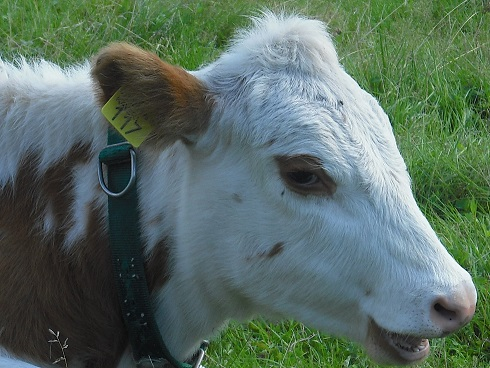
\includegraphics{smile}<>
    \end{lstlisting}
    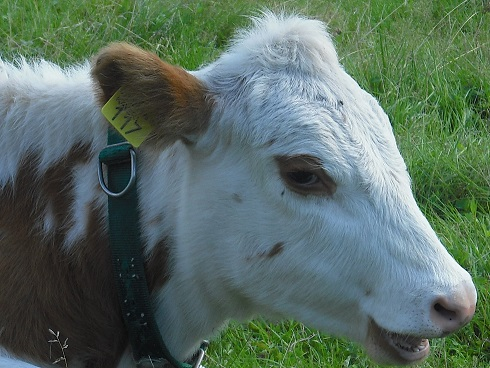
\includegraphics{smile}
\end{frame}

\begin{frame}[fragile]
    \frametitle{Kuvan skaalaus}
    Kuva on aivan liian suuri, joten sitä on syytä skaalata:
    \begin{lstlisting}
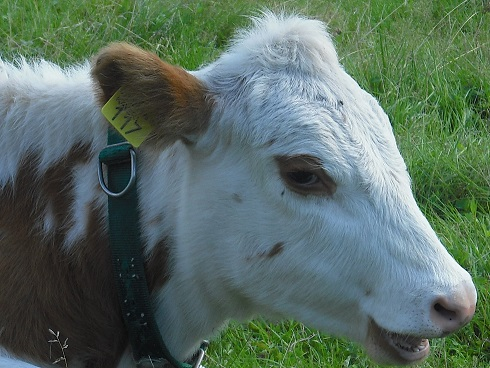
\includegraphics[scale=0.4]{smile}<>
    \end{lstlisting}
    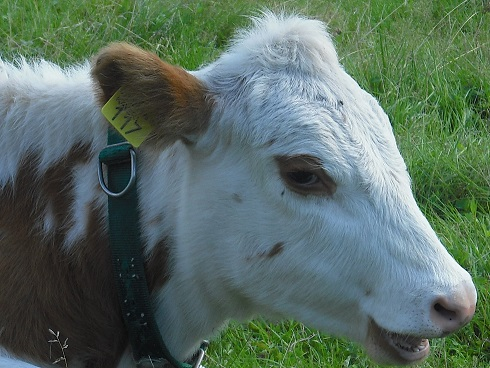
\includegraphics[scale=0.4]{smile}
\end{frame}

\begin{frame}[fragile]
    \frametitle{Kuvan skaalaus}
    Skaalaus onnistuu myös määrittelemällä kuvan leveys tai korkeus:
    \begin{lstlisting}
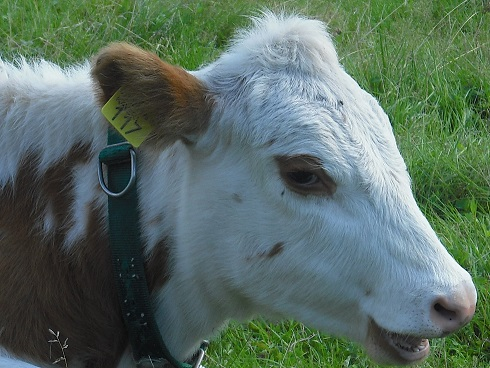
\includegraphics[width = 4cm]{smile}<>
    \end{lstlisting}
    \begin{lstlisting}
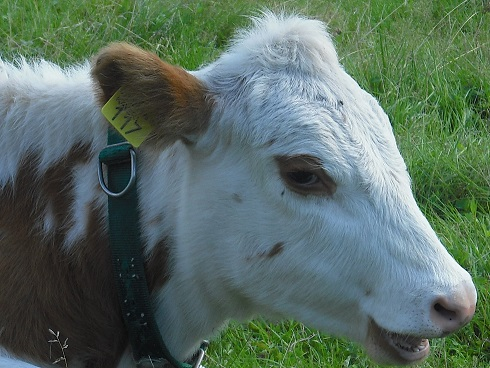
\includegraphics[height=4cm]{smile}<>
    \end{lstlisting}
    \begin{minipage}{5cm}
        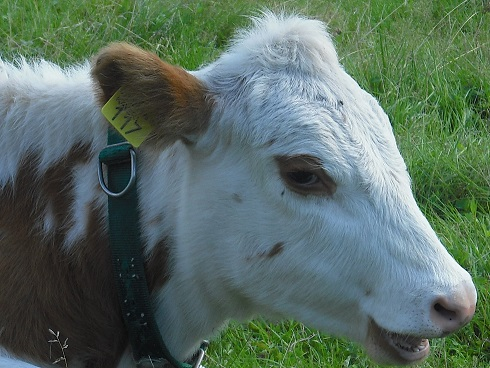
\includegraphics[width = 4cm]{smile}
    \end{minipage}
    \begin{minipage}{5cm}
        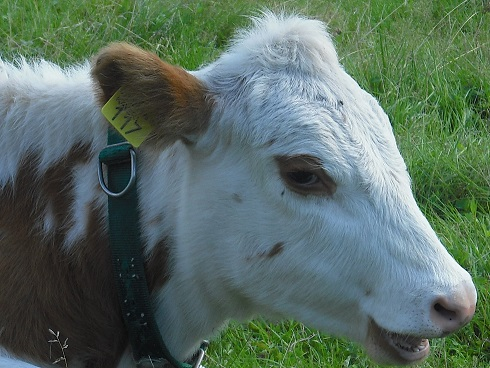
\includegraphics[height=4cm]{smile}
    \end{minipage}
\end{frame}

\begin{frame}[fragile]
    \frametitle{Kuvan kierto}
    Kuvaa voi kiertää antamalla valinnaiseksi argumentiksi kiertokulman asteina.

    \begin{lstlisting}
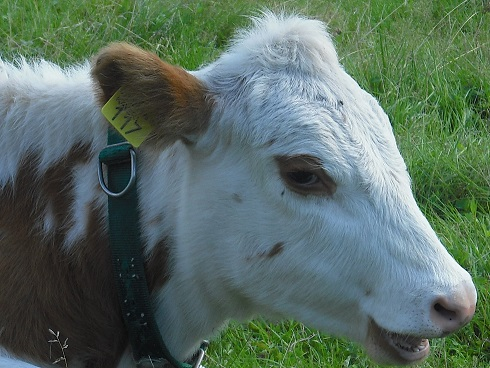
\includegraphics[width=4cm,angle=90]{smile}<>
    \end{lstlisting}
    \begin{lstlisting}
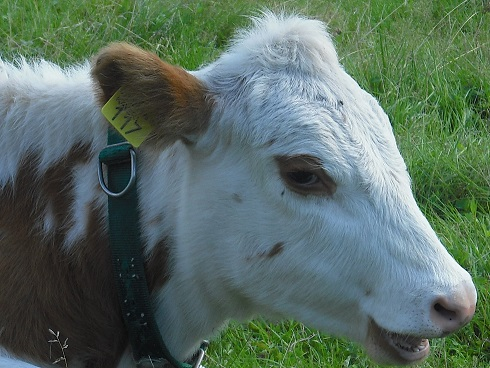
\includegraphics[height=4cm,angle=180]{smile}<>
    \end{lstlisting}
    \begin{minipage}{3cm}
        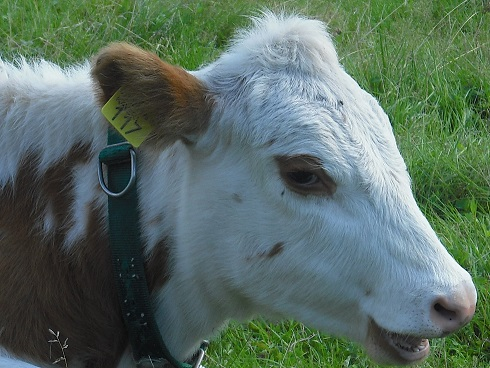
\includegraphics[width = 4cm,angle=90]{smile}
    \end{minipage}
    \begin{minipage}{5cm}
        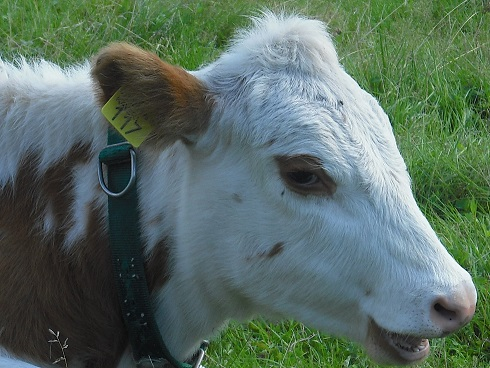
\includegraphics[height=4cm,angle=180]{smile}
    \end{minipage}

    Huomaa, että useammat määritteet erotetaan toisistaan pilkuilla!
\end{frame}

\begin{frame}[fragile]
        \begin{harj}
        Tallenna työkansioosi jokin kuva (tarkkana formaatin kanssa) ja tuo se työhösi sopivasti skaalattuna. Muista ottaa ensin käyttöön paketti \verb-graphicx-! 
    \end{harj}

\end{frame}

\subsubsection{Figure-ympäristö}
\begin{frame}[fragile]
    \frametitle{Kelluva figure-ympäristö}
    Käyttämällä pelkästään komentoa \lstinline-\includegraphics[]{}- kuva tuodaan komennon osoittamaan paikkaan, kuin osaksi tekstiä. Tämä näyttää käytännössä aina pahalta. 
    \vaihto
    On parempi antaa \LaTeX in päättää itse mihin kuva sijoitetaan eli tehdä kuvasta \newterm{kelluva}. Tämä onnistuu käyttämällä \cns{figure}-ympäristöä. 
\end{frame}

\begin{frame}[fragile]
    \frametitle{Kelluva kuva}
    \begin{lstlisting}
\begin{figure}[hb]
    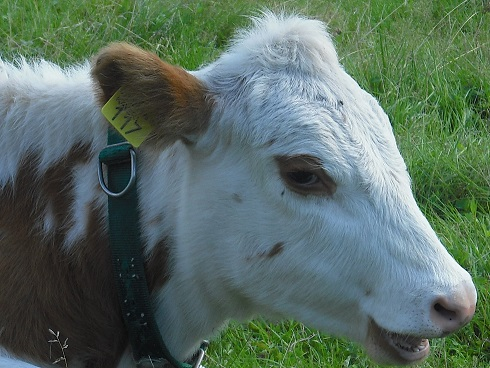
\includegraphics[height=4cm]{smile}
    \caption{Helppo hymyillä}
\end{figure}<>
    \end{lstlisting}
    \begin{figure}[hb]
        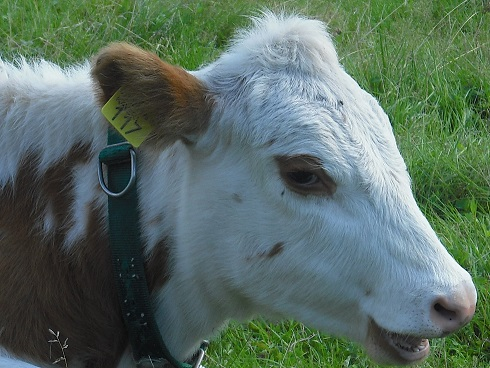
\includegraphics[height=4cm]{smile}
        \caption{Helppo hymyillä}
    \end{figure}
\end{frame}

\begin{frame}[fragile]
    \frametitle{Figure-ympäristön argumentit}
%    Kelluvalle ympäristölle (yllä \verb-figure-) voidaan antaa valinnaisena argumenttina toive kuvan sijoittamisesta. Toiveen voi esittää seuraavilla määritteillä:
    Oletuksena \LaTeX\ yrittää sijoittaa kelluvan ympäristön (yllä \cns{figure}) tekstisivun ylä- tai alareunaan tai sivulle, jolla on vain kelluvia olioita. Valinnaisella argumentilla voi kertoa tarkemmin, mihin kohtaan sijoittaminen \emph{sallitaan}:
    \pause
    \begin{table}
        \begin{tabular}{lcl}

            %h! && tähän\\
            %\hline
            \cns{h} && salli sijoittaminen \emph{tähän} (mahdollisesti keskelle sivua)\\
            \hline
            \cns{t} && salli sijoittaminen (jonkin) sivun yläreunaan\\
            \hline
            \cns{b} && salli sijoittaminen (jonkin) sivun alareunaan\\
            \hline
            \cns{p} && salli sijoittaminen kelluvien otusten sivulle

        \end{tabular}
    \end{table}
    \begin{itemize}[<+->]
        \item Oletuksena on siis \cns{[tbp]}. \pause Pelkkä \cns{[h]} ei ole mahdollinen, vaan korvataan automaattisesti \cns{[ht]}:llä.
        \item Argumenttina voi myös antaa huutomerkin, jolloin \LaTeX\ sallii rumempia lopputuloksia. \pause Esimerkiksi \cns{[!hb]} sallii sijoittamisen tähän tai tekstisivun alareunaan ja lopputulos saa näyttää hieman rumalta.
        \item {\footnotesize Tarkempi (tekninen) kuvaus sijoittelualgoritmista: \url{http://tex.stackexchange.com/a/39020/23378}}
    \end{itemize}
\end{frame}

\begin{frame}[fragile]
    \frametitle{Figure-ympäristön argumentit}
    Usein haluttaisiin sijoittaa kelluva ympäristö \underline{tähän} kohtaan tekstiä \textit{no matter what}. 
    \pause
    \vaihto
    Se onnistuu \cns{float}-paketilla. Tällöin esittelyosaan on lisättävä rivi \lstinline-\usepackage{float}-, jonka jälkeen kelluvalle ympäristölle voi antaa argumentin \verb-[H]-, joka toteuttaa toiveesi, oli jälki miten rumaa tahansa. Argumentin \cns{H} kanssa ei voi käyttää muita; esim. \cns{[Hp]} on laiton yhdistelmä.
    \pause
    \vaihto
        \begin{harj}
        Tuo työhösi jokin kuva käyttäen figure-ympäristöä ja anna valinnaisena argumenttina toiveesi kuvan sijoittamisesta. Lisää vielä kuvateksti.
    \end{harj}

\end{frame}

\subsubsection{Piirtäminen (TikZ)}
\begin{frame}[fragile]
    \frametitle{Kuvien piirtäminen}
    Kuvien liittämisen lisäksi niitä voi myös piirtää suoraan \LaTeX illa. Yksinkertaisimmissa tapauksissa tämä onnistuu helposti, monimutkaisempien kuvien tuottaminen vaatii harjaantumista.
    \vaihto
    Kuvien piirtäminen vie aikaa, mutta jälki on sen mukaista eikä erillisiä kuvatiedostoja tarvitse säilyttää.
    \vaihto Kuvien piirtämistä varten on tarjolla muutamia paketteja, joista erityisesti \TikZ{} on syytä mainita. Runsaasti esimerkkejä (koodeineen) löytyy täältä: \url{http://www.texample.net/tikz/examples/all/}
    \vaihto Geogebra osaa kääntää sillä luodut kuvat \TikZ-koodiksi, mikä helpottaa työtä valtavasti.
    \vaihto Muita kuvien tuottamiseen tarkoitettuja paketteja ovat picture, xy-Pic ja Asymptote.
\end{frame}

\begin{frame}[fragile]
        \begin{harj}
    Piirrä Geogebralla jokin yksinkertainen kuva (vältä funktioita). Rajaa kuva sopivasti ja valitse File > Export > Graphics View as PGF/TikZ. Luo koodi ja kopioi siitä tarvittavat osat tiedostoosi. Tarvittavia osia ovat esittelyosan komennot \verb-\usepackage...-, \verb-\usetikzlibrary...-, mahdolliset värien määrittelyt \verb-\definecolor...- ja varsinainen kuva, eli \verb-\begin{tikzpicture}...\end{tikzpicture}-. 
    \end{harj}

        \begin{harj}\label{kelluvaTikz}
        Kopioi edellisessä harjoituksessa luomasi kuvan koodi ja tee kuvaan joitakin muutoksia pelkästään koodia muuttamalla. Voit esimerkiksi vaihtaa jonkin pisteen paikkaa tai piirtää kokonaan uutta. Tee uudesta kuvasta kelluva ja keksi jokin kuvateksi. 
    \end{harj}

\end{frame}


\subsection{Taulukot}
\begin{frame}[fragile]
    \frametitle{Taulukot}
    Taulukoiden rakentaminen \LaTeX issa on oma taiteenlajinsa. Mahdollisuudet ovat rajattomat, mutta perusteiden opettelu vaatii hieman energiaa. 
    \vaihto
Perinteisin tapa on käyttää \cns{tabular}-ympäristöä. Tällöin taulukon sisältö kirjoitetaan komentojen \lstinline-\begin{tabular}[]{}- ja \lstinline-\end{tabular}- väliin.
    \vaihto
    Ympäristöllä on pakollinen argumentti, jolla määritellään taulukon asetukset, eli miten kunkin sarakkeen sisältö tasataan ja millaisia pystyviivoja käytetään.
\end{frame}

%\begin{frame}[fragile]

%\frametitle{Taulukot}
%Komento 
%\begin{Verbatim}[frame=single]
%\begin{tabular}{cc|c}
%-1 & 2 & 3,142\\
%4 & 5 & -6\\
%0 & 0 & 0
%\end{tabular}
%\end{Verbatim}
%luo taulukon, jossa on yksi pystyviiva ja jonka jokaisen sarakkeen sisältö on keskitetty:
%\begin{framed} 
%\begin{tabular}{cc|c}
%-1 & 2 & 3,142\\
%4 & 5 & -6\\
%0 & 0 & 0
%\end{tabular}
%\end{framed}
%Huomaa, ettei asetuksissa oteta kantaa rivien määrään.
%\end{frame}

\subsubsection{Tabular-ympäristö}
\begin{frame}[fragile]
    \frametitle{Tabular-ympäristö}
    Tabular-ympäristön pakollinen argumentti on jono seuraavia merkkejä:
    \begin{table}
        \begin{small}
            \begin{tabular}{ccl}
                Merkki && Toiminto\\
                \hline
                \cns{r} && sarakkeen sisällön tasaus oikealle\\
                \hline
                \cns{l} && sarakkeen sisällön tasaus vasemmalle\\
                \hline
                \cns{c} && sarakkeen sisällön keskitys\\
                \hline
                \cns{|} && pystyviivan paikka\\
                \hline
                \cns{||} && kaksi pystyviivaa\\
                \hline
                \cns{p\{pituus\}} && pituus, jonka jälkeen rivi katkaistaan\\
                \hline
            \end{tabular}
        \end{small}
    \end{table}
    Esimerkiksi komento \lstinline-\begin{tabular}{r|cc}- aloittaisi 3-sarakkeisen taulukon, jolla olisi pystyviiva 1. ja 2. sarakkeen välillä. Sarakkeen 1 sisältö tasattaisiin oikealle, kahden muun sisältö keskitettäisiin.
    %\vaihto
    %Lisätietoja ympäristön käytöstä saa kirjasta  \begin{scriptsize}\url{http://en.wikibooks.org/wiki/LaTeX/Tables#The_tabular.2A_environment}\end{scriptsize}
\end{frame}

\begin{frame}[fragile]
    \frametitle{Tabular-ympäristö}
    Taulukon sisältö kirjoitetaan rivi kerrallaan. Jokaisella rivillä merkki \lstinline-&- erottaa sarakkeet toisistaan, komennolla \lstinline-\\- siirrytään seuraavalle riville.  Nämä ja muut taulukon sisäiset komennot ovat seuraavassa:
    \vaihto
    \begin{table}
        \begin{small}
            \begin{tabular}{cl}
                Komento & Toiminto\\
                \hline
                \lstinline-&- & sarakkeenvaihto\\
                \hline
                \lstinline-\\- & rivinvaihto\\
                \hline
                \lstinline-\hline- & vaakaviiva \\
                \hline
                \lstinline-\newline- & rivinvaihto sarakkeen sisällä\\
                \hline
                \lstinline+\cline{i-j}+ & vaakaviiva sarakkeiden i ja j välillä\\
                \hline
            \end{tabular}
        \end{small}
    \end{table}
\end{frame}

\begin{frame}[fragile]
    \frametitle{Tabular-ympäristö}
    Esimerkiksi koodi
    \begin{lstlisting}
\begin{tabular}{r|cc}
    & Tytöt & Pojat\\
    \hline
    Sinisilmäiset & 4 & 2 \\
    Ruskeasilmäiset & 3 & 5 \\
    Vihreäsilmäiset & 8 & 8\\
\end{tabular}<>
    \end{lstlisting}
    luo seuraavan taulukon:
    \begin{sample} 
        \begin{tabular}{r|cc}
            & Tytöt & Pojat\\
            \hline
            Sinisilmäiset & 4 & 2 \\
            Ruskeasilmäiset & 3 & 5 \\
            Vihreäsilmäiset & 8 & 8\\
            %\hline
            %Yhteensä: & 15 & 15\\
        \end{tabular}
    \end{sample}
    Huomaa, ettei rivien lukumäärää tarvitse erikseen kertoa \LaTeX ille.
\end{frame}

\begin{frame}[fragile]
    \frametitle{Tabular-ympäristö}
        \begin{harj}
        Laadi jokin 3-sarakkeinen taulukko, jossa on ainakin kaksi riviä.  
        %ja joka sisältää
        %\begin{itemize}
        %\item pystyviivan
        %\item kaksinkertaisen pystyviivan
        %\item vaakaviivan
        %\item osittaisen vaakaviivan sarakkeiden 1 ja 2 välillä
        %\end{itemize}
    \end{harj}

        \begin{harj}
        Luo toinen 3-sarakkeinen taulukko (esim. kopio edellisestä), joka sisältää 
        \begin{itemize}
            \item pystyviivan
            \item kaksinkertaisen pystyviivan
            \item vaakaviivan
            \item osittaisen vaakaviivan kahden sarakkeen välillä
        \end{itemize}
    \end{harj}

\end{frame}

\subsubsection{Sarakkeiden yhdistäminen}
\begin{frame}[fragile]
    \frametitle{Sarakkeiden yhdistäminen}
    Sarakkeiden yhdistäminen onnistuu komennolla \lstinline-\multicolumn{}{}{}-. Pakollisista argumenteista
    \begin{itemize}
        \item ensimmäinen on yhdistettävien solujen lukumäärä
        \item toinen on yhdistämällä saadun sarakkeen tasaus
        \item kolmas on yhdistämällä saadun sarakkeen sisältö
    \end{itemize}
    Komento \lstinline-\multicolumn- toimii sellaisenaan eikä tarvitse lisäpaketteja.
\end{frame}

\begin{frame}[fragile]
    \frametitle{Sarakkeiden yhdistäminen}
    %\begin{minipage}{5cm}
    \begin{lstlisting}
\begin{tabular}{|c|c|c|}
    \hline
    \multicolumn{3}{|c|}{3 yhdistettyä saraketta}\\
    \hline
    Sarake & \multicolumn{2}{c|}{2
                        yhdistettyä saraketta}\\
    \hline
    Sarake1 & Sarake2 & Sarake3\\
    \hline
\end{tabular}<>
    \end{lstlisting}
    %\end{minipage}
    \begin{serif}
        \begin{small}
            \begin{tabular}{|c|c|c|}
                \hline
                \multicolumn{3}{|c|}{3 yhdistettyä saraketta}\\
                \hline
                Sarake & \multicolumn{2}{c|}{2 yhdistettyä saraketta}\\
                \hline
                Sarake1 & Sarake2 & Sarake3\\
                \hline
            \end{tabular}
        \end{small}
    \end{serif}
\end{frame}

\begin{frame}[fragile]
    \frametitle{Sarakkeiden yhdistäminen}

        \begin{harj}
        Luo seuraava taulukko:
        \begin{table}
            \begin{serif}
                \begin{tabular}{|l|l|l|}
                    \hline
                    \multicolumn{3}{|c|}{\Large Päiväpetolintuja}\\
                    \hline
                    \textit{Nimitys} & \textit{Suku} & \textit{Laji}\\ \hline
                    Kanahaukka & Accipiter &  gentilis\\ \hline
                    Hiirihaukka & Buteo & buteo\\ \hline
                    %\multicolumn{3}{|c|}{Jalohaukkoja}\\ \hline
                    Tuulihaukka & Falco & columbarius\\\hline
                    Nuolihaukka & Falco & subbuteo\\ \hline
                \end{tabular}
            \end{serif}
        \end{table}
    \end{harj}

\end{frame}

\subsubsection{Rivien yhdistäminen}
\begin{frame}[fragile]
    \frametitle{Rivien yhdistäminen}
    Rivien yhdistämistä varten tarvitaan paketti \cns{multirow}. Tämän käyttöönottamisen jälkeen rivien yhdistäminen (sarakkeen sisällä) onnistuu komennolla \lstinline-\multirow{}{}{}-. Pakollisista argumenteista
    \begin{itemize}
        \item ensimmäinen on yhdistettävien solujen lukumäärä
        \item toinen on yhdistämällä saadun rivin leveys (\cns{*} jättää asian \LaTeX in huoleksi)
        \item kolmas on yhdistämällä saadun rivin sisältö
    \end{itemize}
    Rivin leveyttä ei useinkaan kannata itse valita, ellei ole varma siitä mitä haluaa tehdä. 
    \vaihto
    Huomaa, että \lstinline-\multirow- toimii kuten \lstinline-\multicolumn-, mutta keskimmäinen argumentti on eri tarkoitusta varten.
\end{frame}

\begin{frame}[fragile]
    \frametitle{Rivien yhdistäminen} 
    \begin{lstlisting}
\begin{tabular}{|c|c|c|}
    \hline
    \multirow{3}{*}{Kolme riviä} & Solu1 & Solu 2\\
    \cline{2-3}
    & \multirow{2}{*}{Kaksi riviä} & Solu 3\\
    \cline{3-3}
    & & Solu 4\\
    \hline
\end{tabular}<>
    \end{lstlisting}
    \begin{serif}
        \begin{small}
            \begin{tabular}{|c|c|c|}
                \hline
                \multirow{3}{*}{Kolme riviä} & Solu1	& Solu 2\\\cline{2-3}
                                              & \multirow{2}{*}{Kaksi riviä}	& Solu 3\\\cline{3-3}
                                              & & Solu 4\\
                \hline
            \end{tabular}
        \end{small}
    \end{serif}
\end{frame}

\begin{frame}[fragile]
    \frametitle{Rivien yhdistäminen} 
        \begin{harj}\label{taulukko}
        Luo seuraava taulukko: 
        \begin{table}
            \begin{serif}
                \begin{tabular}{|c|c|c|c|}
                    \hline
                    \textit{Heimo} & \textit{Nimitys} & \textit{Suku} & \textit{Laji}\\ \hline
                    \multirow{2}{*}{Haukat} & Kanahaukka & Accipiter &  gentilis\\ \cline{2-4}
                                            & Hiirihaukka & Buteo & buteo\\ \hline
                    %\hline
                    %Analyysi I \& II & \multirow{3}{*}{Matikan perusopinnot}\\
                    %\cline{1-1}
                    %Linis I & \\
                    %\cline{1-1}
                    %JYM & \\
                    %\hline
                \end{tabular}
            \end{serif}
        \end{table}
    \end{harj}

\end{frame}

\begin{frame}[fragile]
    \frametitle{Sarakkeiden ja rivien yhdistäminen} 
    Sarakkeita ja rivejä voi yhdistää samassa taulukossa:
    \begin{lstlisting}[basicstyle=\ttfamily\scriptsize]
\begin{tabular}{|l|l|l|l|}
    \hline
    \multicolumn{4}{|c|}{\textbf{Päiväpetolintuja}}\\
    \hline
    \textit{Heimo} & \textit{Nimitys} & \textit{Suku} & \textit{Laji}\\
    \hline
    \multirow{2}{*}{Haukat} & Kanahaukka & Accipiter &  gentilis\\
                              \cline{2-4}
                            & Hiirihaukka & Buteo & buteo\\
    \hline
    \multirow{2}{*}{Jalohaukat} & Tuulihaukka & Falco & columbarius\\
                                  \cline{2-4}
                                & Nuolihaukka & Falco & subbuteo\\
    \hline
\end{tabular}<>
    \end{lstlisting}
    \begin{table}
        \begin{serif}
            \begin{scriptsize}
                \begin{tabular}{|l|l|l|l|}
                    \hline
                    \multicolumn{4}{|c|}{\textbf{Päiväpetolintuja}}\\
                    \hline
                    \textit{Heimo} & \textit{Nimitys} & \textit{Suku} & \textit{Laji}\\\hline
                    \multirow{2}{*}{Haukat} & Kanahaukka & Accipiter &  gentilis\\ \cline{2-4}
                                            & Hiirihaukka & Buteo & buteo\\ \hline
                    \multirow{2}{*}{Jalohaukat} & Tuulihaukka & Falco & columbarius\\ \cline{2-4}
                                                &Nuolihaukka & Falco & subbuteo\\ \hline
                \end{tabular}
            \end{scriptsize}
        \end{serif}
    \end{table}
\end{frame}

\begin{frame}
    Taulukoiden rakentamisessa lähes mikä tahansa on mahdollista. Kirjasta \url{http://en.wikibooks.org/wiki/LaTeX/Tables} voi etsiä apua monimutkaisempia toteutuksia varten.
\end{frame}

%\begin{frame}[fragile]
%\frametitle{Kelluvat taulukot}
%Yleensä taulukot kannattaa esittää kelluvina ympäristöinä. Tämä tarkoittaa sitä, että \LaTeX\ päättää itse, mihin taulukko kannattaa ulkonäöllisesti sijoittaa. Tällöin \verb-tabular--ympäristö sijoitetaan \verb-table--ympäristöön:
%
%\end{frame}
%\begin{frame}[fragile]
%\frametitle{Kelluvat taulukot}
%\verb-table--ympäristölle voidaan antaa valinnaisena argumenttina toive taulukon sijoittumisesta seuraavilla määritteillä:
%\begin{tabular}{cc}
%h! & tähän\\
%h & suunnilleen tähän\\
%b & sivun alareunaan\\
%p & sivun yläreunaan
%\end{tabular}
%\end{frame}

\subsubsection{Kelluva table-ympäristö}
\begin{frame}[fragile]
    \frametitle{Kelluva table-ympäristö}
Komento \lstinline-\begin{tabular}{...}...\end{tabular}- luo taulukon komennon osoittamaan paikkaan, kuin osaksi tekstiä. Tämä näyttää käytännössä aina pahalta. 
    \vaihto
    On parempi antaa \LaTeX in päättää itse mihin taulukko sijoitetaan eli tehdä siitä \emph{kelluva}. Tämä onnistuu sijoittamalla taulukko \cns{table}-ympäristöön.
    \begin{lstlisting}
\begin{table}[H]
    \begin{tabular}{...}
        ...
    \end{tabular}
\end{table}<>
    \end{lstlisting}
    Ympäristön \cns{table} sijoittelu noudattaa samoja sääntöjä kuin \cns{figure} ja sitä voi säätää antamalla ympäristölle valinnaisena argumenttina osan tai kaikki merkeistä \cns{!htbp} (tai \cns{float}-pakettia käyttämällä \cns{H}).
\end{frame}

%\begin{frame}[fragile]
%    \frametitle{Table-ympäristön argumentit}
%    Kelluvalle ympäristölle (yllä \verb-table-) annetaan valinnaisena argumenttina toive taulukon sijoittamisesta. Toiveen voi esittää seuraavilla määritteillä:
%    \begin{table}
%        \begin{tabular}{lcl}
%
%            h! && tähän\\
%            \hline
%            h && suunnilleen tähän\\
%            \hline
%            b && sivun alareunaan\\
%            \hline
%            t && sivun yläreunaan\\
%            \hline
%            p && omalle sivulleen\\
%
%        \end{tabular}
%    \end{table}
%    Toive ei ole \LaTeX in tärkeysjärjestyksessä korkeimmalla, joten se ei aina toteudu.
%\end{frame}

\begin{frame}[fragile]
        \begin{harj}\label{kelluvaTaulukko}
        Tee tehtävässä \ref{taulukko} luomastasi taulukosta kelluva ja anna sille jokin nimi. Kokeile erilaisia sijoitteluvaihtoehtoja. Lisää koodiisi kommenttirivi, jossa kerrot valintasi. 
    \end{harj}

\end{frame}


\subsection{Matriisit}

\begin{frame}[fragile]
    \frametitle{Matematiikkatilan taulukot}
    \LaTeX\ olettaa \cns{tabular}-ympäristön sisältävän tavallista tekstiä. Taulukoituja matemaattisia ilmaisuja varten on oma ympäristönsä \cns{array}. Sitä käytetään kuten \cns{tabular}-ympäristöä, mutta se täytyy sijoittaa matematiikkatilaan.\vaihto

    \begin{minipage}{5cm}
        \begin{lstlisting}
\[
    \begin{array}{r|c}
        x & x^2+1\\
        \hline
        -1 & 2\\
        0 & 1\\
        1 & 2\\
    \end{array}
\]<>
        \end{lstlisting}
    \end{minipage}
    \begin{minipage}{5cm}
        \[
        \begin{array}{r|c}
            x & x^2+1\\
            \hline
            -1 & 2\\
            0 & 1\\
            1 & 2\\
        \end{array}
        \]
    \end{minipage}
\end{frame}

\begin{frame}[fragile]
    \frametitle{Array-ympäristö}
    \cns{array}-ympäristöllä voi kirjoittaa esimerkiksi paloittain määritellyn funktion lausekkeen. Tämän voi toteuttaa lyhyemminkin käyttäen ympäristöä \cns{cases}. 
    \begin{lstlisting}
\[
    f(x) =
    \begin{cases}
        x,  & \text{kun } x>0,\\
        -x, & \text{kun } x\leq0.
    \end{cases}
\]<>
    \end{lstlisting}
    \begin{sample}
        \[
            f(x) =
            \begin{cases}
                x,  & \text{kun } x>0,\\
                -x, & \text{kun } x\leq0.
            \end{cases}
        \]
    \end{sample}
\end{frame}

\subsubsection{Matriisiympäristöt}
\begin{frame}[fragile]
    \frametitle{Matriisit}
    Matriisit voitaisiin luoda käsin käyttäen \cns{array}-ympäristöä, mutta hieman helpompiakin tapoja on. Esimerkiksi ympäristöllä \cns{pmatrix} matriiseja luotaisiin seuraavasti:

    \begin{minipage}{5cm}
        \begin{lstlisting}
\[
    \begin{pmatrix}
        a & b & c\\
        1 & 2 & 3\\
    \end{pmatrix}
\]<>
        \end{lstlisting}
    \end{minipage}
    \begin{minipage}{5cm}
        \[
            \begin{pmatrix}
                a & b & c\\
                1 & 2 & 3\\
            \end{pmatrix}
        \]
    \end{minipage}

    Syntaksi on siis samanhenkinen kuin ympäristöllä \cns{array}, mutta sarakkeiden määrää ei tarvitse kertoa erikseen. Virheiden varalta muista, että
    \begin{itemize}
        \item sarakkeet erotetaan toisistaan merkillä \lstinline-&-
        \item rivi vaihdetaan komennolla \lstinline-\\-
    \end{itemize}

    %\end{frame}
    %\begin{frame}[fragile]
    %
    %\end{frame}
    %loisi matriisin
%Saman voi kuitenkin tehdä helpommin käyttämällä matriiseja varten luotuja ympäristöjä, kuten \verb-bmatrix*- tai \verb-pmatrix*-. Näitä varten tarvitset paketin \verb-mathtools-.
\end{frame}

\begin{frame}[fragile]
        \begin{harj}
        Luo jokin vähintään \(2\times 3\)-matriisi käyttäen ympäristöä \verb-pmatrix-, kuten yllä. Tee sitten matriisistasi muutama kopio ja kokeile ympäristöjä \verb-matrix-, \verb-bmatrix- ja \verb-vmatrix-. (Kunkin kohdalle kannattaa kirjoittaa kommentti tulostuvan matriisin tyylistä.)
    \end{harj}

\end{frame}

\begin{frame}[fragile]
    \frametitle{Matriisit}
    Vaikka ympäristöt \cns{pmatrix} (\cns{matrix}, \cns{bmatrix}, \cns{vmatrix}) pohjautuvat \cns{array}-ympäristöön, ei sarakkeiden tasaukseen voi lähtökohtaisesti vaikuttaa. \vaihto Paketti \cns{mathtools} tarjoaa vastaavat ympäristöt \cns{pmatrix*}, \cns{bmatrix*} jne., joilla on valinnaisena argumenttina sarakkeissa käytetty tasaus:\vaihto

    \begin{minipage}{5cm}
        \begin{lstlisting}
\[
    \begin{pmatrix*}[r]
        a & b & c\\
        -1 & -2 & -3\\
    \end{pmatrix*}
\]<>
        \end{lstlisting}
    \end{minipage}
    \begin{minipage}{5cm}
        \[
            \begin{pmatrix*}[r]
                a & b & c\\
                -1 & -2 & -3\\
            \end{pmatrix*}
        \]
    \end{minipage}
    %Seuraavaan taulukkoon on koottu yleisimmin tarvittavat matriisiympäristöt:
    %\vaihto
    %\begin{tabular}{|c|c|}
    %\hline
    %Ympäristön nimi & Matriisin tyyli\\[0.3em]
    %\hline
    %\verb-matrix*- & $\begin{smallmatrix}a&b\\ c&d\end{smallmatrix}$\\[0.3em]
    %\verb-pmatrix*- & $\bigl(\begin{smallmatrix}a&b\\ c&d\end{smallmatrix} \bigr)$\\[0.3em]
    %\verb-bmatrix*- & $\bigl[\begin{smallmatrix}a&b\\ c&d\end{smallmatrix} \bigr]$\\[0.3em]
    %\verb-vmatrix*- & $\left|\begin{smallmatrix}a&b\\ c&d\end{smallmatrix} \right|$\\[0.3em]
    %\hline
    %\end{tabular}
    %\vaihto
    %Ympäristöllä on valinnainen argumentti, jolla valitaan tekstin tasaus (r, l tai c). Jos ympäristön nimestä jätetään * pois, sarakkeiden sisältö keskitetään (tällöin pakettia \verb-mathtools- ei tarvita). 
\end{frame}

\begin{frame}[fragile]
    \frametitle{Matriisit}

    Esimerkki:\vaihto
    \begin{minipage}{5cm}
        \begin{lstlisting}
\[
    \begin{bmatrix*}[r]
        -1 & 2\\
        0 & 1\\
        1 & -2\\
    \end{bmatrix*}^T = 
    \begin{bmatrix*}[r]
        -1 & 0 & 1\\
        2 & 1 & -2
    \end{bmatrix*}
\]<>
        \end{lstlisting}
    \end{minipage}
    \begin{minipage}{5cm}
        \[
        \begin{bmatrix*}[r]
            -1 & 2\\
            0 & 1\\
            1 & -2\\
        \end{bmatrix*}^T = 
        \begin{bmatrix*}[r]
            -1 & 0 & 1\\
            2 & 1 & -2
        \end{bmatrix*}
        \]
    \end{minipage}
\end{frame}

\begin{frame}[fragile]
    \frametitle{Matriisit}
        \begin{harj}
        Kirjoita seuraavanlainen matriisitoimitus: 
        \begin{align*}
            &
            \begin{bmatrix*}[r]
                0 & 0 & 1 & a_1\\
                0 & 1 & 1 & a_2\\
                1 & 1 & 1 & a_3
            \end{bmatrix*}
%        \stackrel{\begin{scriptsize} R_1\leftrightarrow R_3 \end{scriptsize} }{\longrightarrow}
        \xrightarrow{R_1\leftrightarrow R_3}
            \begin{bmatrix*}[r]
                1 & 1 & 1 & a_3\\
                0 & 1 & 1 & a_2\\
                0 & 0 & 1 & a_1
            \end{bmatrix*}
            %\\
            %\stackrel{\begin{scriptsize} R_1-R_2 \end{scriptsize} }{\longrightarrow}
            %&\begin{bmatrix*}[r]
            %1 & 0 & 0 & a_3-a_2\\
            %0 & 1 & 1 & a_2\\
            %0 & 0 & 1 & a_1
            %\end{bmatrix*}
            %\stackrel{\begin{scriptsize} R_2-R_3 \end{scriptsize} }{\longrightarrow}
            %\begin{bmatrix*}[r]
            %1 & 0 & 0 & a_3-a_2\\
            %0 & 1 & 0 & a_2-a_1\\
            %0 & 0 & 1 & a_1
            %\end{bmatrix*}
        \end{align*}
        Matriisien sisällön saat päättää vapaasti eikä rivitoimituksen tarvitse mennä oikein. % Matriisien välisen merkinnän saat rakennettua komennon \verb-\stackrel{}{}- avulla. Yllä on käytetty komentoa
        Kaavan mukana automaattisesti venyvän nuolen saa komennolla \lstinline-\xrightarrow{kaava}-.
%        \begin{verbatim}
%        \stackrel{
%            \begin{scriptsize} 
%                R_1\leftrightarrow R_3 
%            \end{scriptsize}
%        }{\longrightarrow} 
%        \end{verbatim}

        % Kannattaa kopioida alkuperäisen matriisin koodi ja muokata sitä kunkin uuden matriisin kohdalla. Matriisit vievät paljon tilaa, joten ympäristö \verb-align*- on hyödyksi!
    \end{harj}

\end{frame}

\subsubsection{Lisätietoa}
\begin{frame}[fragile]
    \frametitle{Lisätietoa matriiseista}
    Tavalliset matriisiympäristöt \cns{pmatrix} jne. voidaan säätää noudattamaan paremmin \cns{array}-ympäristön syntaksia.
    \vaihto
    Tämä on tarpeen, jos halutaan valita eri sarakkeisiin erilainen tasaus tai luoda pystyviiva matriisin sisälle. 
    \vaihto
    Syntaksin muuttaminen onnistuu kopioimalla esittelyosaan komennot\vaihto
    \begin{lstlisting}
\makeatletter
\renewcommand*\env@matrix[1][*\c@MaxMatrixCols c]{%
    \hskip -\arraycolsep
    \let\@ifnextchar\new@ifnextchar
\array{#1}}
\makeatother<>
    \end{lstlisting}
\end{frame}

\begin{frame}[fragile]
    \frametitle{Lisätietoa matriiseista}
    Edellä tehtyjen muutosten jälkeen matriisiympäristöt toimivat kuten ennenkin, mutta lisäksi valinnainen argumentti on käytössä kuten \cns{array}-ympäristöllä:
    \vaihto
    \begin{minipage}{6cm}
        \begin{lstlisting}
\[
    \begin{bmatrix}[rrr|r]
        0 & 0 & 1 & -a_1\\
        0 & 1 & -1 & a_2\\
        1 & 1 & 1 & a_3
    \end{bmatrix}
\]<>
        \end{lstlisting}
    \end{minipage}
    \begin{minipage}{4cm}
        \[
            \begin{bmatrix}[rrr|r]
                0 & 0 & 1 & -a_1\\
                0 & 1 & -1 & a_2\\
                1 & 1 & 1 & a_3
            \end{bmatrix}
        \]
    \end{minipage}
\end{frame}



\section{4.kerta}


\subsection{Viittaaminen kuviin ja taulukoihin}

\begin{frame}[fragile]
    \frametitle{Viittaaminen kuviin ja taulukoihin}
    Kelluviksi kirjoitetut kuvat ja taulukot tulevat numeroiduiksi, jolloin niihin viittaaminen onnistuu helposti komennoilla \lstinline-\label{}- ja \lstinline-\ref{}-. 
    %\begin{itemize}
    %\item \verb-\ref{nimi}- (tulostaa viitattavan kohteen numeron)
    %\item \verb-\eqref{nimi}- (tulostaa kohteen numeron sulkujen sisällä)
    %\item \verb-\pageref{nimi}- (tulostaa sen sivun numeron, jolla kohde on)  
    %\end{itemize}
    %Sisäisten viittausten kanssa tulee aina käyttää komentoja. Tällöin viittaukset pysyvät kohdallaan vaikka numeroinnit muuttuisivat työn edetessä.
    %\end{frame}
    %\begin{frame}[fragile]
    %Huom! Uuden viittauksen jälkeen työn joutuu ajamaan kahdesti, jotta numeroinnit tulevat näkyviin (kahden kysymysmerkin sijaan).
        \begin{harj}
        Viittaa harjoituksessa \ref{kelluvaTaulukko} luomaasi kelluvaan taulukkoon. Käytä komentoja \lstinline-\ref{}- ja \lstinline-\pageref{}-. Komento \lstinline-\label{..}- tulee taulukkoon liittyvän \lstinline-\caption{..}--komennon jälkeen.
        %\vaihto
        %Muista, että viitattavalle kohteelle on ensin annettava tunnus komennolla \verb-\label{valitsemasi tunnus}-. Komento sijoitetaan ympäristön aloittavan komennon \verb-\begin{}- perään.
    \end{harj}

        \begin{harj}
        Sama kuin edellinen harjoitus, mutta viittaa harjoituksessa \ref{kelluvaTikz} luomaasi kelluvaan kuvaan.
    \end{harj}

\end{frame}


\subsection{Kirjallisuusviitteet}

\subsubsection{Lainaukset ja alaviitteet}
\begin{frame}[fragile]
    \frametitle{Lainaukset ja alaviitteet}
    Suomalaisittain käytettävät lainausmerkit saa kahdella peräkkäisellä \lstinline-'- merkillä:
    \begin{lstlisting}
Matti sanoi: ''Onpa outoa!''<>
    \end{lstlisting}
    tulostaa
    \begin{sample}
        Matti sanoi: ''Onpa outoa!''
    \end{sample}
    Lainauksia varten on olemassa myös omia ympäristöjään, kuten \cns{verse}, \cns{quote} ja \cns{quotation}.
    \vaihto
    Alaviitteen voi luoda komennolla \lstinline-\footnote{teksti}-. Komento kirjoitetaan siihen kohtaan, johon alaviitteen merkki halutaan. 
\end{frame}

\begin{frame}[fragile]
        \begin{harj}
        Lisää dokumenttiisi jokin lainaus käyttäen \verb-quote--, \verb-\quotation-- tai \verb-verse--ympäristöä. 
    \end{harj}

        \begin{harj}
        Lisää työhösi alaviite komennolla \lstinline-\footnote{}-. 
    \end{harj}

\end{frame}

\subsubsection{\BibTeX-järjestelmä}
\begin{frame}[fragile]
    \frametitle{Kirjallisuusviitteet}
    \LaTeX issa kirjallisuusviittaukset kannattaa hoitaa \BibTeX-järjestelmän avulla. 
    \vaihto
%    Tällöin jokaista lähdeteosta kohden luodaan erillinen \verb-.bib--tiedosto, joka sisältää teoksen tiedot. 
    Tällöin lähdeteokset kirjataan erilliseen \cns{.bib}-tiedostoon (tai -tiedostoihin).
    \vaihto
    Tiedostot on yksinkertaisinta tallentaa samaan kansioon \cns{.tex}-tiedoston kanssa.
    \vaihto
    Viittaaminen tapahtuu komennolla \lstinline-\cite{tunnus}-, jossa \cns{tunnus} on eräs \cns{.bib}-tiedostosta löytyvä merkkijono.
    %\vaihto
    %Aivan työn loppuun luodaan kirjallisuusluettelo komennoilla
    %\begin{Verbatim}[frame=single]
    %\bibliographystyle{luettelon tyyli}
    %\bibliography{teos1.bib, teos2.bib, teos3.bib,...}
    %\end{Verbatim}
    %Edellytyksenä on, että tiedostot teos1.bib jne. ovat samassa kansiossa \verb-.tex--tiedoston kanssa.
\end{frame}

\begin{frame}[fragile]
    \frametitle{.bib-tiedostot}
    \cns{.bib}-tiedoston voi luoda millä tahansa tekstieditorilla, erityisen hyvin Texmakerilla. 
    \vaihto
    Tiedoston sisältö voisi olla esimerkiksi seuraava:\vaihto
    \begin{lstlisting}[language=BibTeX,basicstyle=\ttfamily\small]
@book{kemper,
    title={A Course in Commutative Algebra},
    author={Kemper, G.},
    isbn={9783642035456},
    series={Graduate Texts in Mathematics},
    url={http://books.google.fi/books?id=8kxlj48DWM4C},
    year={2010},
    publisher={Springer Berlin Heidelberg}
}<>
    \end{lstlisting}
    %Tiedosto tallennetaan muodossa \verb-jokinNimi.bib- samaan kansioon \verb-.tex--tiedoston kanssa (ei pakollista, mutta yksinkertaisinta).
\end{frame}

\begin{frame}[fragile]
    \frametitle{.bib-tiedostot}
        \begin{harj}
        Kopioi edellisen esimerkin sisältö uuteen tiedostoon ja tallenna se nimellä \cns{lahteet.bib} työkansioosi. 
    \end{harj}

\end{frame}

\begin{frame}[fragile]
    \frametitle{.bib-tiedoston sisältö}
    \begin{itemize}
        \item Ensimmäisellä komennolla (\lstinline[language=BibTeX]-@book-, \lstinline[language=BibTeX]-@article-, \lstinline[language=BibTeX]-@unpublished- jne.) kerrotaan, minkä tyyppisestä teoksesta on kyse. 
        \item Aaltosulkeisiin ennen ensimmäistä pilkkua tuleva merkkijono on se tunnus, jolla teokseen viitataan komennolla \lstinline-\cite{tunnus}-. 
        \item Tunnuksen voi valita vapaasti (ilman ääkkösiä ja erikoismerkkejä) eikä se tule näkyviin mihinkään.  Esimerkiksi yllä tunnus on \cns{kemper}, joten teokseen viitattaisiin komennolla \lstinline-\cite{kemper}-.
        \item Muut kentät (ja niiden pakollisuus/valinnaisuus) määräytyvät teoksen tyypin mukaan.
    \end{itemize}
\end{frame}

\begin{frame}[fragile]
    \frametitle{Luokat ja .bib-tiedoston sisältö}
    Kun tiedostoja luodaan käsin, täytyy selvittää mitkä kentät ovat pakollisia ja mitkä valinnaisia. 
    \vaihto
    Esimerkiksi taulukosta 
    \begin{scriptsize}
        \url{http://en.wikibooks.org/wiki/LaTeX/Bibliography_Management#Entry_and_field_types_in_.bib_files}
    \end{scriptsize}
    selviää, että kirjalle (\lstinline[language=BibTeX]-@book-) pakollisia kenttiä ovat \cns{title} ja \cns{author}, muut valinnaisia.
    \vaihto
    Lisätietoa käytettävistä teosluokista löytyy esimerkiksi sivulta
    \begin{scriptsize}
        \url{http://en.wikibooks.org/wiki/LaTeX/Bibliography_Management#Standard_templates}.
    \end{scriptsize}
    \vaihto
    Käytännössä jokaista kuviteltavissa olevaa lähdeteosta varten löytyy jokin sopiva luokka (ja tarpeen tullen sellaisen voi luoda itsekin).
\end{frame}

\begin{frame}[fragile]
        \begin{harj}
        Lisää tiedostoon \cns{lahteet.bib} kirja, jonka nimi on Topologia I, kirjoittaja Jussi Väisälä, julkaisija Limes ry ja painovuosi 2000. Valitse viittaustunnukseksi \cns{topo1}.
    \end{harj}

\end{frame}

\begin{frame}[fragile]
    \frametitle{.bib-tiedostot Internetistä}
    Kirjojen teostietoja löytää \BibTeX -muodossa varsin suurella todennäköisyydellä Google Books-palvelusta. 
    \vaihto
    Kuhunkin teokseen liittyvän Tietoja teoksesta-sivun alalaidassa on kohta Vie sitaatti ja sen vieressä painike \BibTeX, josta tiedoston voi ladata.
    \vaihto
    Tiedosto kannattaa avata Texmakerillä, tehdä mahdolliset muutokset ja tallentaa haluttuun kansioon. 
    \vaihto
    Käytännössä ainakin viittaustunnus on syytä vaihtaa helpommaksi.
\end{frame}

\begin{frame}[fragile]
    \frametitle{.bib-tiedostot Internetistä}
        \begin{harj}
        Etsi Google Books-palvelusta Walter Rudinin kirjan Complex Analysis (kirjan versiolla ei väliä) tiedot \BibTeX -muodossa. Avaa tiedosto Texmakerilla ja valitse viittaustunnus haluamaksesi. Tallenna tiedosto nimellä \verb-Rudin.bib- työkansioosi. (Huomaa, että palvelu tarjoaa tiedostot muodossa .bibtex.)
    \end{harj}

\end{frame}

\begin{frame}[fragile]
    \frametitle{Kirjallisuusluettelon luominen}
    Kun tarvittavat \cns{.bib}-tiedostot on tallennettu koneelle, on syytä luoda kirjallisuusluettelo. Kirjallisuusluetteloon tulee näkyviin ne teokset, joiden tiedot ovat olemassa ja joihin on viitattu ainakin kerran. Ei-viitatun teoksen saa lisättyä lähdeluetteloon \lstinline-\nocite{tunnus}--komennolla.
    \vaihto
    Luettelo luodaan työn loppuosaan komennoilla
    \begin{lstlisting}
\bibliographystyle{luettelon tyyli}
\bibliography{lista1,lista2,lista3,...}<>
    \end{lstlisting}
    Koodissa \cns{lista\textit{x}} ovat \cns{.bib}-tiedostojen nimet ilman \cns{.bib}-päätettä. Huomaa myös, ettei pilkun jälkeen sallita välilyöntiä.
    \vaihto
    Edellisen koodin toimimisen edellytyksenä on, että tiedostot \cns{lista1.bib} jne. ovat samassa kansiossa \cns{.tex}-tiedoston kanssa. 
\end{frame}

\begin{frame}[fragile]
    \frametitle{Kirjallisuusluettelon luominen}
        \begin{harj}
        Edellä loit \BibTeX-tiedostot \verb-lahteet.bib- ja \verb-Rudin.bib-. Tuo teokset kirjallisuusluetteloon koodilla 
        \begin{Verbatim}[frame=single]
\bibliographystyle{plain}
\bibliography{lahteet,Rudin}
        \end{Verbatim}
        Sijoita koodi työsi loppuosaan, esimerkiksi juuri ennen komentoa \verb-\end{document}-.
    \end{harj}

        \begin{harj}
        Viittaa kuhunkin teokseen työssäsi komennolla \lstinline-\cite{viittaustunnus}-.
    \end{harj}

\end{frame}
\begin{frame}[fragile]
    \frametitle{Käytäntö}
    %Kun tiedostot on luotu ja tallennettu, niihin voidaan viitata tuloksellisesti jo mainitulla komennolla \verb-\cite{tunnus}-. 
    Jotta viitteet tulisivat näkyviin, toimi seuraavasti:
    \begin{itemize}
        \item aja tiedosto PDFLaTeXilla
        \item aja tiedosto \BibTeX{}illa (ja tarkista alapalkkiin ilmestyvät viestit!)
        \item aja tiedosto PDFLaTeXilla kahdesti
    \end{itemize} 
    Jos viittaukset eivät tule näkyviin etkä tiedä mistä se johtuu, tarkista seuraavat kohdat:
    \begin{itemize}
        \item oletko käyttänyt viitatessa oikeita tunnuksia?
        \item oletko tuonut tiedostot \LaTeX iin oikein ja oikeilla nimillä?
        \item ovatko tiedostot todella muotoa \cns{.bib}?
        \item ovatko tiedostot oikeassa kansiossa?
    \end{itemize}
\end{frame}

\begin{frame}[fragile]
    \begin{extra}
        \begin{itemize}
            \item Viittauksen lisäämisen/poistamisen/muuttamisen jälkeen ensimmäinen \LaTeX-ajo merkitsee löytyneet viittaustunnukset \cns{.aux}-tiedostoon.
            \item Tämän jälkeen \BibTeX-ajo kirjoittaa \cns{.aux}-tiedoston perusteella lähdeluettelon tuottavan \LaTeX-koodin \cns{.bbl}-tiedostoon.
            \item Seuraava \LaTeX-ajo lukee myös \cns{.bbl}-tiedoston koodin, jolloin lähdeluettelo tulee näkyviin (jos sitä ei vielä ole) ja viittaustiedot lisätään/päivitetään \cns{.aux}-tiedostoon.
            \item Viimeinen \LaTeX-ajo osaa nyt \cns{.aux}-tiedoston perusteella korvata kysymysmerkit oikeilla viittauksilla.
        \end{itemize}
    \end{extra}
\end{frame}
%\begin{frame}[fragile]
%\frametitle{Viittaustyyli}
%%\begin{harj}
%Luo tai etsi Internetistä kolmelle eri teokselle \BibTeX-tiedostot ja viittaa teoksiin onnistuuneesti. Valitse teoksille eri luokat, esim \verb-@book-, \verb-@misc- ja \verb-@unpublished-.
%\end{harj}

%\end{frame}
\subsubsection{Viittaustyyli}
\begin{frame}[fragile]
    \frametitle{Viittaustyyli}
    Viittaukset tulevat näkyviin hakasuluissa olevina numeroina. Esimerkiksi lähdeteoksen kirjoittajaa varten lukija joutuu siis tarkistamaan lähdeluettelon. Tämä on tyypillistä varsinkin matemaattisessa kirjallisuudessa. 
    \vaihto
    Toisenlaista viittaustekniikkaa varten voi käyttää esimerkiksi \cns{natbib}-järjestelmää, jota ei kuitenkaan tällä kurssillä käsitellä. Lisätietoa saa vaikkapa osoitteesta
    \begin{scriptsize}
        \url{http://en.wikibooks.org/wiki/LaTeX/Bibliography_Management#Natbib}
    \end{scriptsize}
\end{frame}


\subsection{Dokumentin viimeistely}

\subsubsection{Sisällysluettelo ja kansilehti}
\begin{frame}[fragile]
    \frametitle{Sisällysluettelo ja kansilehti}
    Sisällysluettelon saa haluamaansa kohtaan työtä komennolla \lstinline-\tableofcontents-. Tiedoston joutuu yleensä ajamaan useaan kertaan, ennen kuin numeroinnit tulevat näkyviin oikein.
    \vaihto
    Kansilehti luodaan komennolla \lstinline-\maketitle-. Tätä varten esittelyosaan lisätään komennot \lstinline-\title{otsikko}-, \lstinline-\author{nimi}- ja haluttaessa \lstinline-\date{pvm}-. Päivämäärän saa pois komennolla \lstinline-\date{}-.
    \vaihto
    Kansilehti tulostuu joissain luokissa (esim. \cns{book} ja \cns{report}) omaksi sivukseen, \cns{article}-luokassa osaksi ensimmäistä sivua.
\end{frame}

\begin{frame}[fragile]
        \begin{harj}
        Luo työllesi kansilehti ja sisällysluettelo. Kokeile miltä työsi näyttää, jos vaihdat luokaksi \cns{report} tai \cns{book}. Millaisia eroja huomaat? 
    \end{harj}

        \begin{harj}
        Dokumenttia on helpompi navigoida elektronisesti, kun viitteet toimivat linkkeinä. Ota tätä varten käyttöön paketti \cns{hyperref}. Kokeile kääntää dokumentti -- linkkien ympärillä on nyt ruma laatikko. Paranna tilannetta antamalla \cns{hyperref}-paketille argumentti \cns{colorlinks=true} (ota mallia esim. \cns{inputenc}-paketin lataavasta rivistä).
    \end{harj}

\end{frame}

\subsubsection{Dokumenttiluokan asetukset}
\begin{frame}[fragile]
    \frametitle{Dokumenttiluokan asetukset}
    Tiedoston aloittavalle komennolle \lstinline-\documentclass[]{}- voi antaa valinnaisena argumenttina eräitä dokumentin ulkoasua koskevia asetuksia:
    \begin{itemize}
        \item Kirjainkoon vaihtoehdot ovat \cns{10pt}, \cns{11pt} ja \cns{12pt}. 
        \item Luonnostilan saa valinnalla \cns{draft}. Tällöin kääntäminen on nopeaa ja liian pitkät rivit tulevat merkityiksi.
        \item Tekstin saa jaettua kahteen kolumniin valinnalla \cns{twocolumn}. 
        \item article-luokassa tulostus on oletusarvoisesti yksipuoleinen -- tämän voi vaihtaa valinnalla \cns{twoside} (vast. \cns{oneside}).
    \end{itemize}
    Useammat määritteet erotetaan toisistaan pilkuilla, kuten tavallista.
    \vaihto
    Hieman lisätietoa löytyy esimerkiksi osoitteesta \begin{scriptsize}
        \url{http://texblog.org/2013/02/13/latex-documentclass-options-illustrated}.
    \end{scriptsize}
\end{frame}
%
\end{document}

